%----------------------------------------------------------------------------------------
% PACKAGES AND OTHER DOCUMENT CONFIGURATIONS
% WARNING: Don't mess with any of the following unless you know what you are doing.
%----------------------------------------------------------------------------------------
\documentclass[english,12pt,a4paper,openany]{book}
\usepackage{datetime}
\usepackage{tabularx}
\usepackage{makecell}
\usepackage{eurosym}
\usepackage{pbox}
\usepackage[utf8]{inputenc}
\usepackage[T1]{fontenc}
\usepackage[english]{babel}
\usepackage{amsmath}
\usepackage{amsfonts}
\usepackage{fancyhdr}
\usepackage{amssymb}
\usepackage[dvipsnames]{xcolor}
\usepackage{mdframed}
\usepackage{multirow}
\usepackage{multicol} 
\usepackage{tikz}
\usepackage{graphicx}
\usepackage[absolute]{textpos} 
\usepackage{colortbl}
\usepackage{array}
\usepackage{geometry}
\usepackage{hyperref}
\pagestyle{fancy}
\renewcommand\headrulewidth{1pt}
\usepackage{float}
\usepackage{titlesec}
\hypersetup{hidelinks}

%------------------------------------------------------------------------------------------------------
%	The following are the RGB values for the official ATU colours.
%------------------------------------------------------------------------------------------------------	
\definecolor{ATUGreen}{RGB}{0, 91, 94}
\definecolor{ATULightGreen}{RGB}{172, 245, 189}
\definecolor{ATUNavy}{RGB}{0, 26, 121}
\definecolor{ATUOrange}{RGB}{255, 121, 30}
\definecolor{ATUPurple}{RGB}{77, 8, 87}
\definecolor{ATUSand}{RGB}{255, 232, 212}
\definecolor{ATUTeal}{RGB}{123, 185, 203}
\definecolor{ATUWarmGrey}{RGB}{200, 190, 191}
\definecolor{ATUYellow}{RGB}{248, 255, 142}



%------------------------------------------------------------------------------------------------------
%	******* CHANGE THE FOLLOWING VARIABLES
%------------------------------------------------------------------------------------------------------	

\newcommand{\reportauthor}{Rohan Sikder} % Change to your name
\newcommand{\projecttitle}{TrafficVision}
\newcommand{\reporttype}{Minor Dissertation} %Report  type (Project Plan / Final Report)
\newdateformat{monthyeardate}{\monthname[\THEMONTH], \THEYEAR}


%------------------------------------------------------------------------------------------------------	
% WARNING: Don't mess with any of the following unless you know what you are doing.
%------------------------------------------------------------------------------------------------------	
\pagestyle{fancy}
\fancyhf{}
\fancyhead[R]{\textcolor{ATUGreen}{\reportauthor}}
\fancyhead[L]{\textcolor{ATUGreen}{\projecttitle}}
\fancyfoot[L]{\textcolor{ATUGreen}{Atlantic Technological University (ATU), Galway.}}
\fancyfoot[R]{\thepage}

\begin{document}
\begin{titlepage}

\newgeometry{left=6cm,bottom=2cm, top=1cm, right=1cm}

\tikz[remember picture,overlay] \node[opacity=1,inner sep=0pt] at (2.2mm,-165mm){
\includegraphics{images/leftbar.png}}; % Fond changeable 

\fontfamily{fvs}\fontseries{m}\selectfont
\color{black}

\begin{picture}(0,0)
\put(-110,-743){\rotatebox{90}{\Huge{B.Sc. (Hons) in Software Development}}}
\end{picture}
 
\vspace{-10mm} 

\flushright 
\includegraphics[width=100mm]{images/atu-logo-green.png} 

\flushright
\vspace{10mm}
\textcolor{ATUGreen}{
\fontfamily{cmss}\fontseries{m}\fontsize{22}{26}\selectfont
\projecttitle
}
\normalsize
\color{black}

\vspace{1.5cm}
\normalsize
\textbf{By \\ \textcolor{ATUGreen}{\reportauthor}}\\ 
\vspace{15mm}
{\scshape \today} \\[0.3\baselineskip]
\vspace{75mm}
\Large {\textcolor{ATUGreen}{\textbf{{\reporttype}}}} \\
\bigskip
\normalsize
\textbf{Department of Computer Science \& Applied Physics,\\School of Science \& Computing,\\Atlantic Technological University (ATU), Galway.}\\
\end{titlepage}
\newpage
\tableofcontents
\listoffigures
\pagenumbering{arabic} 
%----------------------------------------------------------------------------------------
%	   ******* CHANGE the Chapters if necessary. Each chapter is encapsulated inside 
%                 its own file. The chapters below are based on the guidelines 
%                 given in the lecture.
%----------------------------------------------------------------------------------------
\chapter{Introduction}
This dissertation presents TrafficVision, a new web application developed to show bus system reliability and punctuality for public transport. Consistent bus schedules result in issues for commuters, the infrastructure and the environment of cities in urbanized areas where efficient transportation is a core element of everyday life. TrafficVision is built for these challenges with computer vision and web technologies, providing real-time information about bus service schedules and quality.

\section{Context and Relevance}

Urban mobility relies on public transportation, particularly bus systems. Their effective operation impacts the environmental sustainability and the daily life of the population. However, bus services often have delays and unpredictability that inconvenience passengers and lead to higher carbon emissions and congestion. Such inefficiencies hinder sustainable urban living. TrafficVision hopes to ease these issues by offering real time bus info so commuters, transportation authorities and urban planners can make the best choice possible.

\section{Project Objectives}

The primary objectives of TrafficVision are:

\begin{itemize}
    \item To develop a web-based platform that offers real-time tracking and analysis of bus services.
    \item To enhance the punctuality and reliability of public transportation through data-driven insights.
    \item To improve the daily commuting experience by minimizing uncertainty and wait times for bus passengers.
    \item To assist in reducing traffic congestion and carbon footprint through efficient bus service management.
\end{itemize}

These objectives form the benchmarks against which the project's success will be evaluated, with specific metrics detailed in the subsequent chapters.

\section{Dissertation Overview}

This dissertation reports on the development of TrafficVision from concept to implementation, highlighting its challenges and creative solutions. It is structured into several key sections:

\begin{itemize}
    \item \textbf{Chapter 1: Introduction} This chapter introduces TrafficVision, a web application aiming to improve public transport reliability by providing real-time bus service data. It outlines the urban mobility challenges and the project’s objectives to enhance bus service punctuality, improve commuting experiences and support sustainable urban living.
    
    \item \textbf{Chapter 2: Methodology} The methodology chapter details the structured approach to software development adopted for the TrafficVision project, including the use of Kanban boards and Gantt charts for project management, Agile methodologies for iterative development and the use of GitHub for collaboration and version control.
    
    \item \textbf{Chapter 3: Technology Review} In this chapter, the technology choices for TrafficVision are justified, including the use of MongoDB for its flexible data schema and cloud integration, Python for computer vision tasks, YOLOv8 over TensorFlow for efficient real-time object detection, React for UI development and Node.js for server-side scripting.

    \item \textbf{Chapter 4: System Design} This chapter covers the system architecture and design, explaining the use of React for front-end deployment, serverless architecture for the processing server, Kafka for data flow management, MongoDB for data storage and the integration of these technologies to create a scalable and responsive system.

    \item \textbf{Chapter 5: System Evaluation} The system evaluation chapter assesses TrafficVision against its initial objectives, presenting results and discussing the system's strengths and limitations. It examines real-time traffic monitoring capabilities, the reliability of public transportation data provided, user engagement and interaction with the system and areas for future development.

    \item \textbf{Chapter 6: Conclusion} The conclusion revisits the project's context and objectives, summarizing key findings from the system evaluation, the challenges faced and the innovative solutions implemented. It encapsulates the project’s achievements and the potential for future work to enhance the TrafficVision system.

\end{itemize}

\section{Project Resources}

The project's source code and resources are available on GitHub, which served as the code repository throughout the development process. The repository URL is:

\begin{center}
\url{https://github.com/ConorPadraigMurphy/FYP}
\end{center}

The repository contains the following main elements:

\begin{itemize}
    \item \textbf{Codebase} - The complete source code for the TrafficVision application, including frontend, backend and computer vision components.
    \item \textbf{Documentation} - A comprehensive set of documentation detailing the system's setup, deployment and usage instructions.
    \item \textbf{Issue Tracker} - A record of issues, enhancements and tasks managed throughout the project lifecycle.
\end{itemize}
\chapter{Methodology of Software Development}

\section{Roadmaps and Kanban Boards}
The workflow was effectively managed and visualized using Kanban boards in the project. From initial development phases to final testing, each task was represented by a card on the Kanban board in columns labelled To Do,'' In Progress,'' Testing,'' and Done.'' This method allowed an overview of project progress and fast identification of bottlenecks. Additionally, roadmaps were created to describe the overall strategy and project milestones. These roadmaps defined the steps towards short-term and long-term goals and ensured that development followed the project goals. The Kanban board used for the TrafficVision project can be accessed at \url{https://rohansikder4.atlassian.net/jira/software/projects/KAN/boards/1}, providing a real-time view of project management and task progression.

\begin{figure}[H]
    \centering
    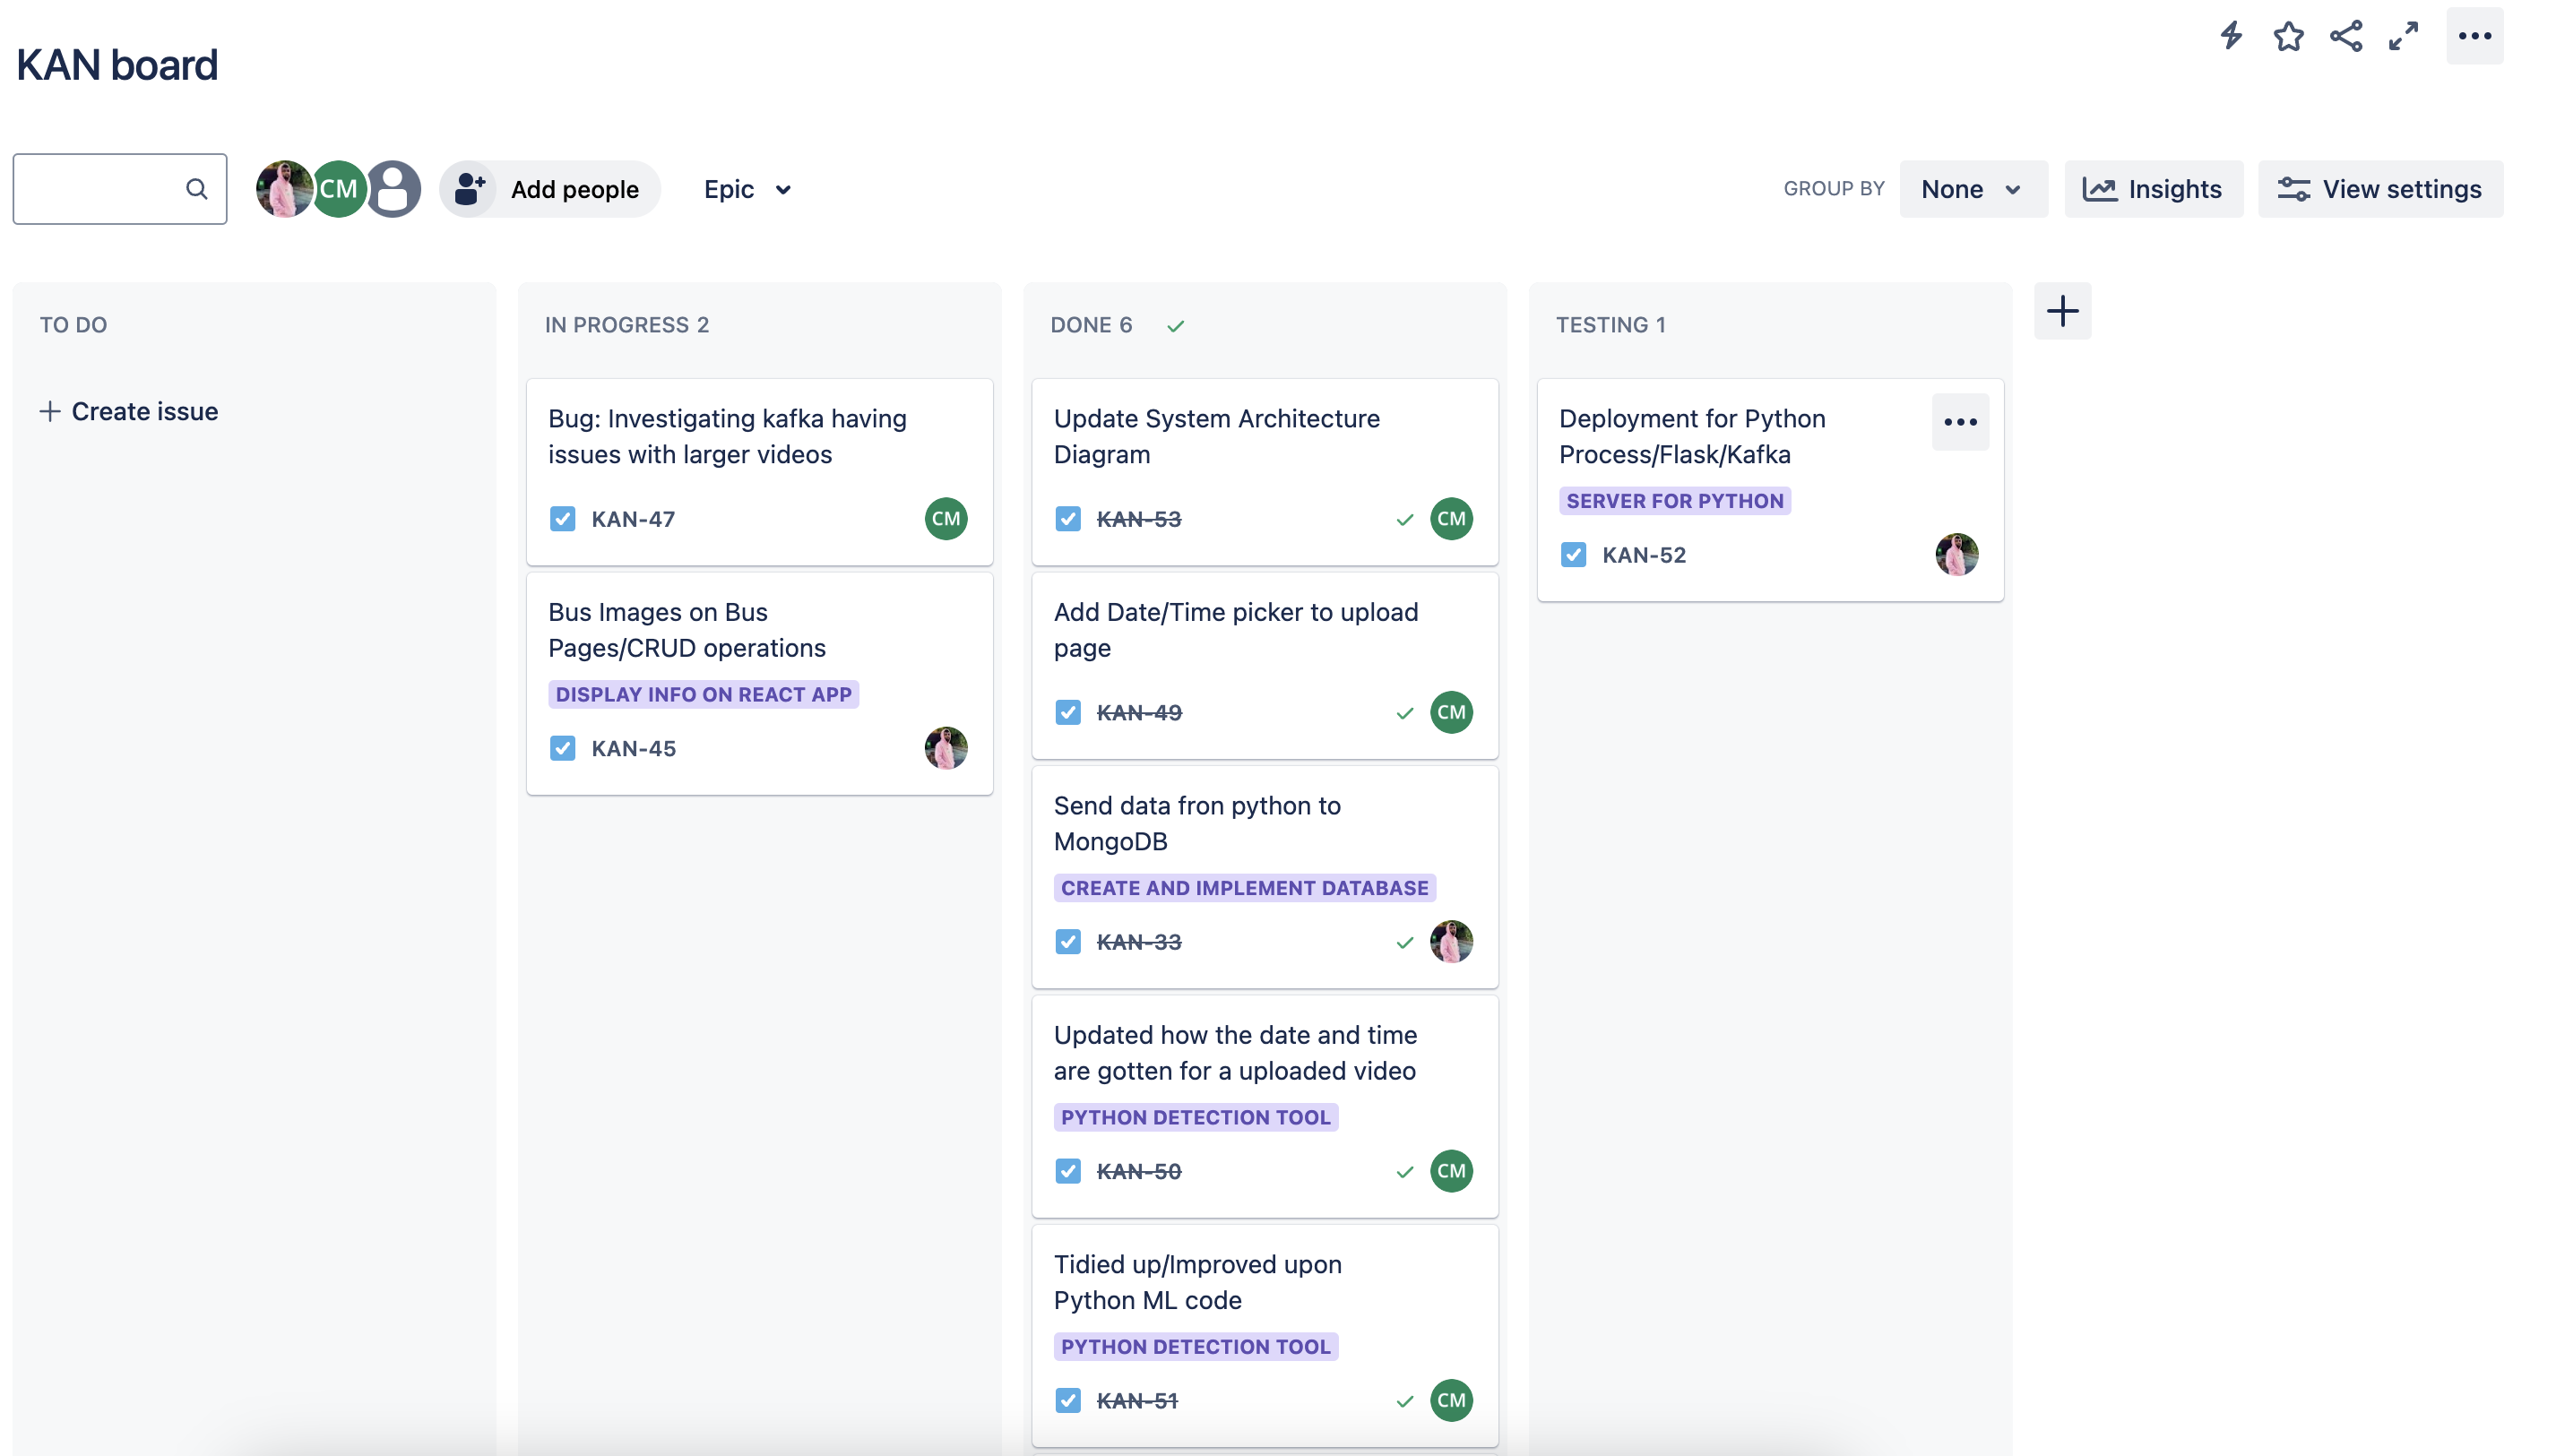
\includegraphics[width=0.8\textwidth]{images/kanban.png}
    \caption{A Screenshot of the Kanban Board.}
    \label{fig:Kanban Board}
\end{figure}


\section{Gantt Chart Integration}
To complement the agile project management approach and enhance visibility into the project timeline, a Gantt chart was employed. This tool was essential in planning, coordinating and tracking specific tasks against time. The Gantt chart for TrafficVision, available at \url{https://rohansikder4.atlassian.net/jira/software/projects/KAN/boards/1/timeline}, illustrates the project’s timeline, including start and end dates for tasks, dependencies and milestones. This visual representation aided in ensuring that project deliverables were completed on schedule and that any potential delays were promptly addressed.


\begin{figure}[h!]
    \centering
    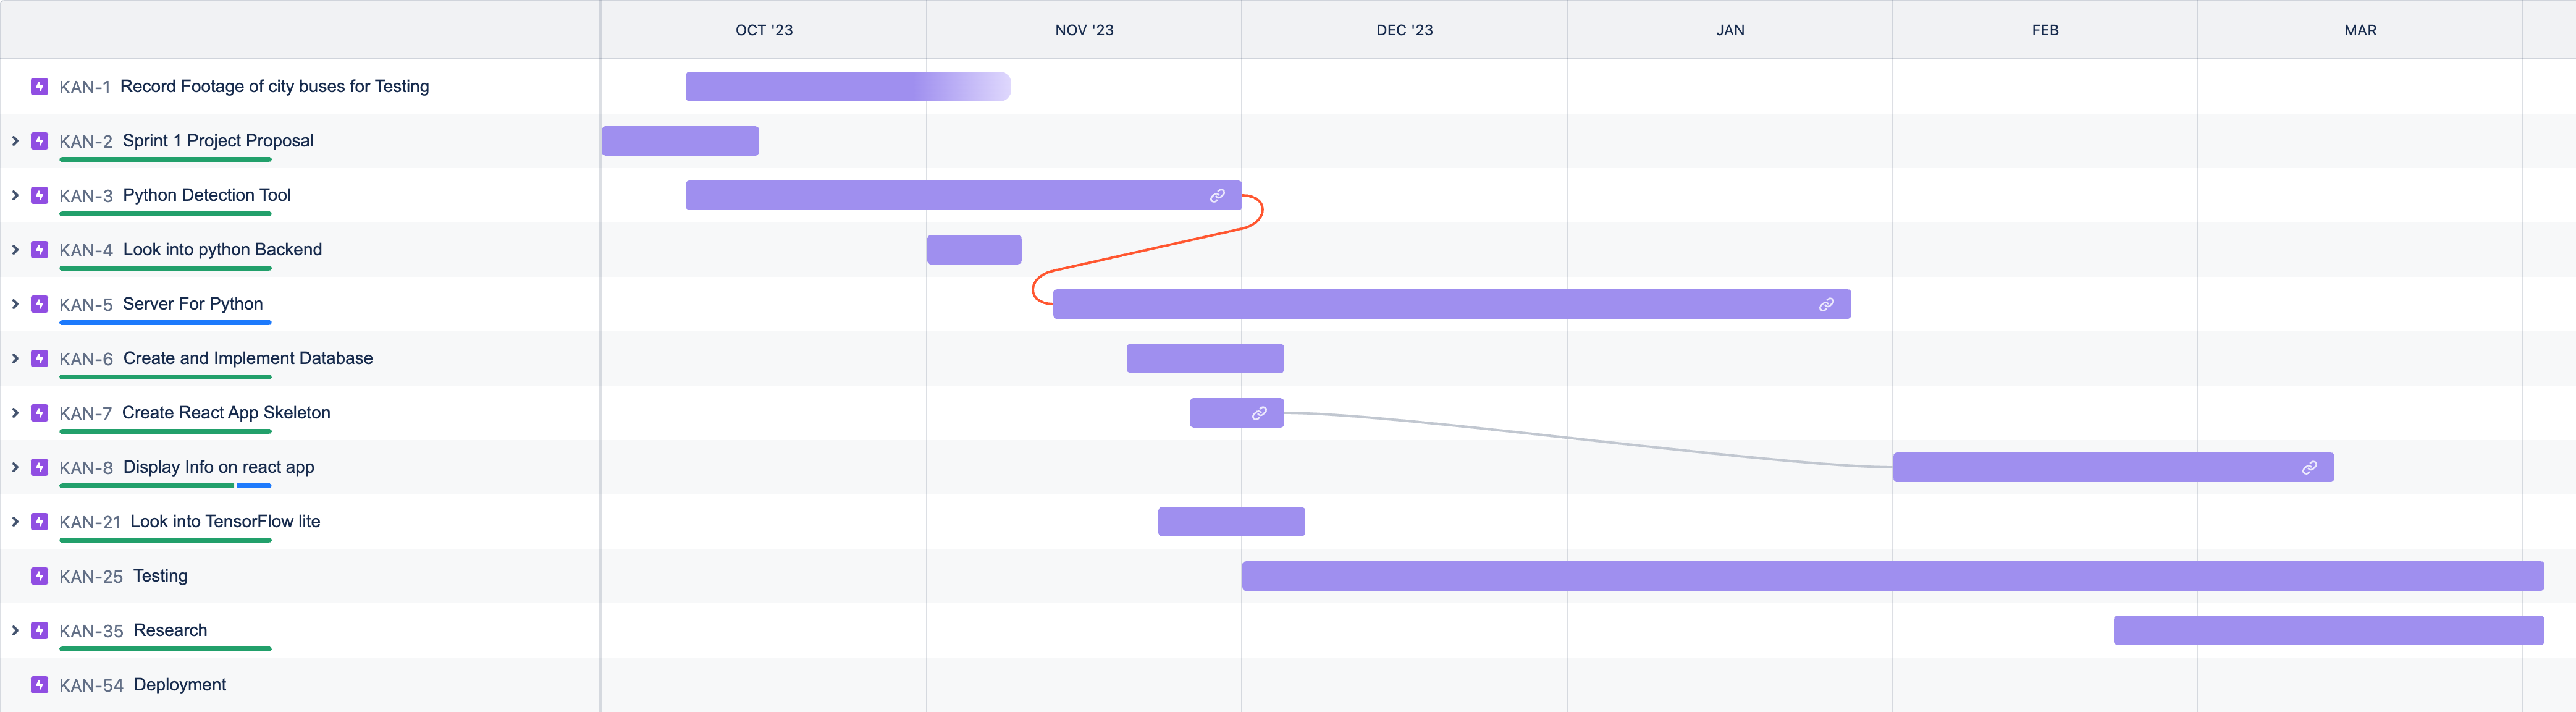
\includegraphics[width=0.8\textwidth]{images/timeline.png}
    \caption{A Gantt Chart which was set out in the beginning of the development proccess.}
    \label{fig:Gantt Chart}
\end{figure}


\section{Agile Methodologies}
While primarily Kanban-based, the project also included elements of Agile\cite{agilemanifesto2001} methodology with emphasis on iterative development and adaptability. Sprint meetings regularly reviewed progress, solved problems and planned future tasks, allowing for rapid iterations on the project scope based on real-time information and feedback.

\section{Meetings and Communication}

Effective communication was essential to the project. Regularly scheduled meetings facilitated continuous project problem-solving and iterative development.

\begin{itemize}
    \item \textbf{Weekly Supervisory Meetings:} Weekly Meetings were held with the project supervisor to review progress and plan future tasks and address immediate issues. These meetings ensured the project met its objectives and offered opportunities for mentorship and guidance. Discussions often revolved around both strategic decisions and technical challenges for a comprehensive project oversight.

    \item \textbf{Weekly Planning Sessions:} Along with supervisory meetings, the team conducted Planning Sessions to outline work for the week. These sessions were critical in clarifying goals, identifying roadblocks and reallocating resources as needed to meet project milestones.

    \item \textbf{Code Review Meetings:} When new Code was written, team members scheduled special Meetings to Review the written Code. These sessions focused on assessing code quality, checking functionality meets project requirements and adding for knowledge sharing and learning. Such reviews helped to maintain high code quality and allowed for group ownership of the project.

    \item \textbf{Issue Resolution Discussions:} Any issues noted during the week or in code reviews were promptly addressed in private discussion sessions. These discussions were essential to troubleshooting issues, brainstorming solutions and delivering fixes on time to avoid project delays.
    
\end{itemize}


\section{Collaboration Tools}
The project used various tools to improve communication and productivity. GitHub\cite{github2024} became the central repository for version control and source code management and was used for reviewing work, facilitating collaboration among team members, regardless of their physical location. This integration of GitHub within the development process underscores its importance as a tool for code collaboration and version control in modern software development.

\section{Rationale for Technology Stack}
The project's choice of MongoDB, Python, React and Node.js as its technology stack was driven by their capabilities to deliver a high-performance web application. Each technology was selected for its strengths in specific areas of the project, from data management to user interface development, ensuring both efficiency and scalability.


\section{Validation and Testing}

Ensuring the quality and reliability of TrafficVision was carried throughout the development process. To achieve this, a comprehensive testing strategy was adopted, employing a mix of manual and automated testing approaches to cover the application's frontend, backend and integration points comprehensively.

\subsection{API Testing with Postman}

Postman\cite{postman2021} was especially important for backend validation, specifically the APIs that execute data transactions between the frontend and the database. A popular API test tool, Postman, allowed to simulate client-side requests to the server and check responses for correctness and performance. By writing structured tests in Postman to ensure all endpoints provided expected functionality, returned appropriate status codes and handled edge cases gracefully. This testing ensured that the server-side logic was robust, fault tolerant and ready to deliver intended user interactions.

\subsubsection{Benefits and Outcomes}
The use of Postman for API testing brought several benefits:
\begin{itemize}
    \item \textbf{Rapid Feedback:} Quick feedback to reduce the time to detect and fix issues.
    \item \textbf{Improved Quality:} Consistent API testing led to higher quality software.
    \item \textbf{Enhanced Reliability:} Load and security testing ensured the APIs could handle real-world usage effectively.
\end{itemize}

\begin{figure}[h!]
    \centering
    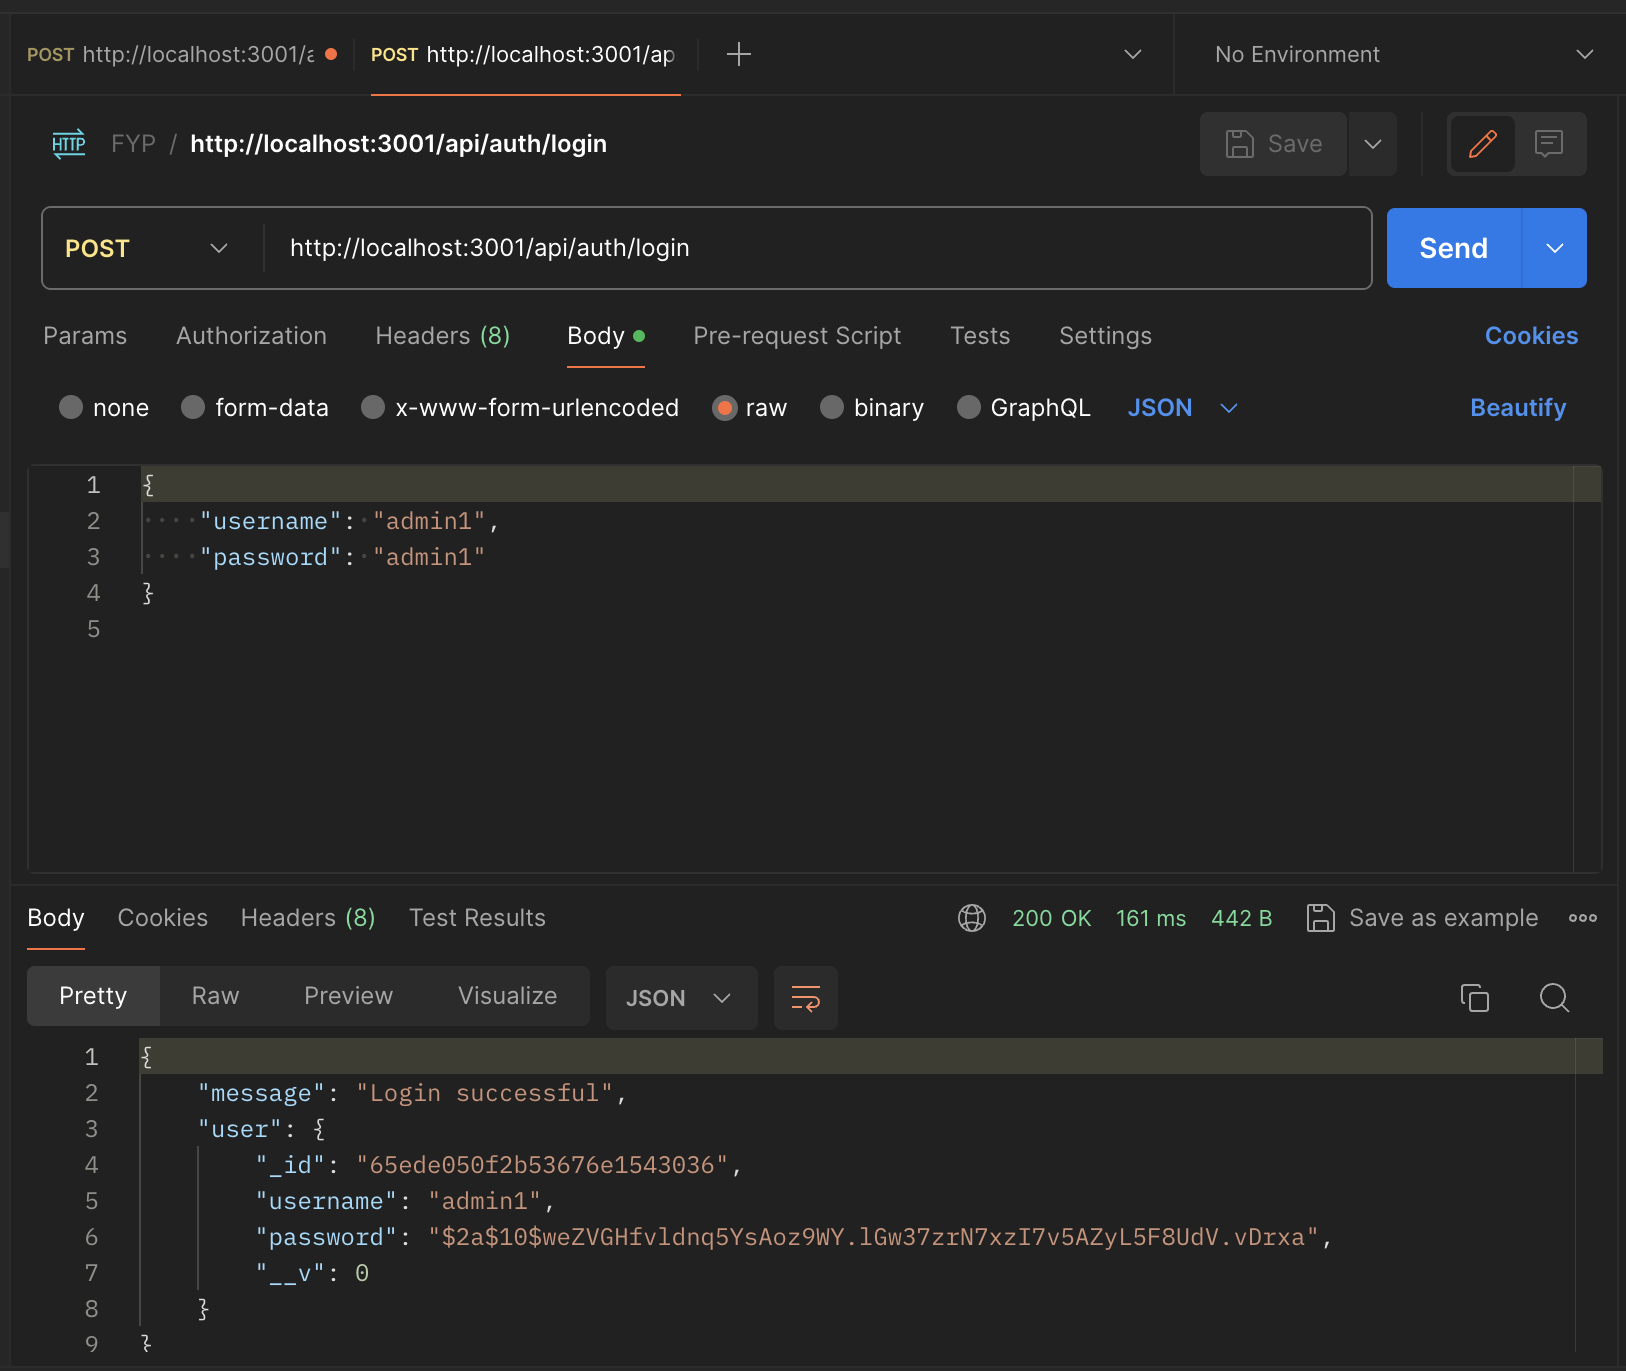
\includegraphics[width=0.8\textwidth]{images/postmanLogin.png}
    \caption{A Postman test demonstrating successful user login API call.}
    \label{fig:postman_login_test}
\end{figure}

\subsection{Developer-Led Frontend Testing}

The frontend was developed with React and tested extensively by the developers that created it. This phase was primarily user testing focusing on the responsiveness, functionality and usability of the user interface. Developers carried out user interactions, navigated the application's features and examined the system behavior in real time. This approach allowed for fast detection and resolution of UI bugs or inconsistencies to ensure intuitive and seamless user experience.

This hands-on testing was complemented by incorporating the frontend and backend services to validate that data flow and processing across system layers worked as intended. This involved testing the real time data display, user authentication and traffic data submission and retrieval.

\subsection{Ensuring Application Robustness}

The combination of Postman for API testing and developers hands-on testing methodology for the frontend meant both critical parts of the TrafficVision application were tested. This methodology allowed for early detection of issues and created quality control.

The project's commitment to testing methodologies emphasized the need to provide a robust and bug-free application capable of enhancing public transportation systems efficiency and reliability. Future enhancements will include additional automated testing frameworks to expand the testing process and coverage to ensure TrafficVision continues to exceed user expectations.


\chapter{Technology Review}

\section{Deeper dive into Technology Selection}

\subsection{MongoDB: Flexibility and Cloud Integration} MongoDB's\cite{mongodb2021} schema-less nature offers the flexibility required for managing diverse data types, including geographical information and user profiles. Its horizontal scalability and robust cloud integration, especially with MongoDB Atlas, made it the preferred choice over traditional SQL databases like MySQL, despite their reliability lacked the same level of flexibility and required additional management for the data. 

\subsection{Python: Optimal for Computer Vision} Python\cite{vanrossum2009} was chosen primarily for its extensive support in computer vision and machine learning tasks, thanks to libraries like OpenCV\cite{bradski2000opencv} and PyTorch. This made it exceptionally suited for implementing the YOLOv8 algorithm for real-time vehicle detection and tracking. While C++ could offer performance advantages, Python's balance of performance, ease of use and large library ecosystem presented the best fit for the project's needs. 

\subsection{Choosing YOLOv8\cite{redmon2018yolov3} over TensorFlow for Object Detection} For the task of real-time vehicle detection and tracking, the project chose YOLOv8, based on the algorithm's faster speed and good object detection accuracy. YOLOv8, the latest YOLO series release, provides faster image processing for real-time applications. This feature is critical for TrafficVision, where timely data processing affects the system performance for traffic monitoring. Though TensorFlow with its object detection API is a powerful and flexible framework that provides several pre-trained object detection models, including some based on the YOLO architecture, YOLOv8 was chosen due to its native video feed processing efficiency. YOLOv8's optimized model architecture minimizes computational consumption without sacrificing the sensitivity required for vehicle identification and tracking under varying lighting and weather conditions. Moreover, YOLOv8's simplified integration with the Python ecosystem made it easier to integrate into the project backend than TensorFlow's custom object detection setup. This ease of integration, combined with Python's deep support for other project requirements, justified moving forward with YOLOv8 for TrafficVision.

\textbf{Summary:} YOLOv8 was selected over TensorFlow due to the project's focus on real-time processing performance, performance and integration ease. Using the strengths of YOLOv8, TrafficVision achieves its goal of real time traffic monitoring, thereby increasing public transportation reliability. 

\subsection{React: Industry Standard for UI Development} The decision to use React\cite{react2021} for developing the user interface was influenced by its widespread adoption and the extensive ecosystem surrounding it. Its component-based architecture simplifies the development of dynamic and responsive web applications. Although alternatives such as Angular and Vue.js were considered, React's flexibility, supported by a large community provided a more suitable solution for TrafficVision's interactive features. 

\subsection{Node.js: Efficient Server-Side Scripting} Node.js\cite{nodejs2024} was selected for its non-blocking, event-driven architecture, ideal for handling TrafficVision's real-time data processing requirements. Its seamless integration with JavaScript for both client and server-side development offers a unified development experience. Despite the availability of other backend frameworks like Django and Spring, Node.js stood out for its lightweight nature and scalability. 


\textbf{Summary:} This carefully selected technology stack ensures that TrafficVision leverages modern, efficient solutions to address the challenges of real-time traffic monitoring and enhancing public transportation systems. The combination of MongoDB, Python, React and Node.js not only caters to the current project requirements but also sets a solid foundation for future scalability and enhancements.


\section{Advanced Urban Traffic Monitoring with OpenCV and YOLOv8 in TrafficVision}
TrafficVision's application of OpenCV and YOLOv8 represents a forefront approach in enhancing urban traffic surveillance through computer vision. This section includes the specific use of these technologies within the TrafficVision framework that showcase the project's innovative capabilities in traffic analysis and management.

\subsection{Using OpenCV: The Foundation for Video Processing}
At the core of TrafficVision's video data processing lies OpenCV, which is utilized to carry out preliminary video processing tasks essential for preparing data for detailed analysis.
\begin{itemize}
    \item \textbf{Frame Extraction and Resizing}: Video frames are extracted from the uploaded streams using OpenCV and resized to a uniform resolution of 640x420 pixels. This standardization ensures consistent analysis across varying video inputs and optimizes the YOLOv8 model's performance by balancing detail against computational efficiency.
\end{itemize}

\subsection{YOLOv8: Pioneering Object Detection and Tracking}
Following initial processing with OpenCV, YOLOv8 undertakes the task of vehicle detection and tracking in the video frames, demonstrating significant advancements in real-time object recognition and tracking.
\begin{itemize}
    \item \textbf{Real-time Object Recognition}: YOLOv8 excels in fast and accurate detection of vehicles within each frame, capable of distinguishing between different vehicle types. This ability allows TrafficVision to accurately classify and enumerate various vehicles, contributing to a comprehensive assessment of traffic composition.

    \item \textbf{Vehicle Tracking Through Frames}: YOLOv8 extends its functionality to track detected vehicles across frames, thereby facilitating an analysis of traffic flow patterns, speeds and potential congestion points. This continuous tracking is integral to understanding traffic dynamics and aids in effective traffic data.
\end{itemize}

\subsection{Integration with Kafka for Real-Time Analysis}
Kafka\cite{kreps2011kafka} is key in managing TrafficVision's data flow, creating the backbone for real-time data streaming and processing. The integration of Kafka demonstrates how TrafficVision leverages event-driven architectures for efficient video data management.
\begin{itemize}
    \item \textbf{Event-driven Architecture}: Upon video upload, the associated metadata is encapsulated in a JSON object and transmitted to a Kafka topic named "incoming-videos". This event-driven methodology underscores Kafka's strength in facilitating scalable and real-time data pipelines.

    \item \textbf{Decoupling of Data Ingestion and Processing}: Through Kafka, TrafficVision achieves a decoupled architecture, allowing video ingestion and processing tasks to scale independently. This separation ensures the system's resilience and adaptability to fluctuating video data volumes.
\end{itemize}

\subsection{Storing Analysis Results in MongoDB}
The analytical outcomes, including vehicle counts, types and direction, are stored in MongoDB. Opting for this NoSQL database aligns with the project's need for scalable and flexible data storage solutions, capable of accommodating schema-less traffic analysis results.

\subsection{YOLOv8 Conclusion}
The integration of OpenCV and YOLOv8 within TrafficVision showcases a high-performance framework for real-time urban traffic analysis. By combining these cutting-edge computer vision technologies with Kafka's data management capabilities and MongoDB's dynamic storage solutions, TrafficVision presents a comprehensive approach to addressing urban traffic challenges. This detailed examination of TrafficVision's technological framework highlights its utilization of leading-edge tools to revolutionize traffic monitoring and management.

\addtocontents{toc}{\protect\newpage}

\section{Flask Framework in TrafficVision's Backend Infrastructure}
The Flask framework serves as a cornerstone in the development of TrafficVision's backend infrastructure, facilitating the seamless creation and management of RESTful API services. This section dives into how Flasks functionality of TrafficVision, from handling video uploads to integrating with Kafka and MongoDB for real-time data streaming and storage.

\subsection{Flask - Streamlining Video Uploads}
At the heart of TrafficVision's Flask application is the capability to handle video uploads, a critical feature for the traffic data pool.
\begin{itemize}
    \item \textbf{Video Upload Endpoint}: Flask's robust routing enables the definition of the `/upload' endpoint, where incoming video files are validated and processed. This ensures that each file is correctly formatted and present, showcasing Flask's efficiency in managing user inputs.
    
    \item \textbf{Data Management}: Utilizing Python's uuid module, Flask assigns a custom video ID to each upload, demonstrating the framework's ability for intricate data management tasks essential for applications dealing with substantial user inputs.
\end{itemize}

\subsection{Implementing Kafka for Real-Time Data Handling}
The integration of Kafka with Flask illustrates a sophisticated approach to real-time data streaming and processing within TrafficVision.
\begin{itemize}
    \item Flask facilitates the encapsulation of video metadata into JSON objects, which are then published to a specific Kafka topic, initiating the asynchronous video data analysis pipeline. This highlights Flask's versatility in supporting microservices architectures and maintaining a scalable, decoupled system design.
\end{itemize}

\subsection{Enhancing Data Management with MongoDB}
Flask's adaptability extends to its integration with MongoDB, emphasizing the framework's capacity to support varied backend functionalities.
\begin{itemize}
    \item By acting as the intermediary between video processing logic and MongoDB, Flask enables the efficient storage and querying of traffic analysis output. This exemplifies Flask's role in projects that require advanced data management capabilities for handling and retrieving extensive datasets.
\end{itemize}

\subsection{Supporting Large Backend Solutions}
TrafficVision's backend architecture, powered by Flask, showcases the framework's strengths in developing scalable and maintainable solutions.
\begin{itemize}
    \item The project leverages Flask's lightweight and modular nature to achieve high efficiency and flexibility in backend services. Flask's design ensures that complexity does not compromise the simplicity of implementing API endpoints.
\end{itemize}

\subsection{Flask Conclusion}
The deployment of Flask within TrafficVision underscores the framework's efficacy in creating agile, scalable and efficient backend services for web applications. By using Flask for video upload functionalities, real-time data streaming with Kafka and data storage with MongoDB, TrafficVision establishes a robust backend infrastructure that not only fulfills present requirements but is also made for future expansion. This utilization of Flask highlights its critical role in the development and success of the TrafficVision project.


\section{Apache Kafka Integration in TrafficVision}
Apache Kafka's integration into TrafficVision exemplifies the application of real-time data streaming and event-driven architectures in urban traffic management systems. By leveraging Kafka, TrafficVision addresses complex requirements for data ingestion, processing and distribution, enhancing the system's ability to manage and interpret vast amounts of traffic data efficiently. This section outlines the specific use cases of Kafka within TrafficVision, emphasizing its critical role in facilitating real-time analytics and integration with other key technologies such as Flask, MongoDB and YOLOv8.

\subsection{Kafka for Data Ingestion and Distribution}
Kafka acts as the cornerstone of TrafficVision's data ingestion and distribution system, channeling video data and analytical results across various application components. Implemented within a Flask-based backend the Kafka producer interfaces with new video streams, recording essential metadata such as video ID, geolocation coordinates and timestamps alongside the actual video content. This setup showcases Kafka's capability to handle high-throughput data streams, allowing TrafficVision to scale its data ingestion efforts in response to fluctuations in traffic video data volumes.

\subsection{Data Processing Workflows: Decoupling}
A distinguishing characteristic of Kafka is its ability to decouple data producers from consumers, a feature that TrafficVision capitalizes on. By using Kafka topics as queues for incoming video data, the architecture allows the video processing unit to function independently of the data ingestion process. This separation enhances the system's availability and resilience, facilitating independent scaling of the video processing workload from data ingestion, thereby optimizing computational resource utilization.

\subsection{Integrating Kafka with Flask and MongoDB}
In TrafficVision, Kafka is utilized not only for data ingestion but also to initiate downstream processing activities. Upon the upload of a video, its metadata is dispatched to a Kafka topic, triggering the activation of the video processing unit. This unit, leveraging YOLOv8 for object detection and tracking, subsequently stores the processed data in MongoDB. The synergy between Kafka, Flask and MongoDB underscores Kafka's role as a robust message broker for asynchronous task execution, contributing to a modular and scalable architectural design.

\subsection{Traffic Analysis in Real Time with YOLOv8}
The real-time traffic analysis capability of TrafficVision is dependent on the YOLOv8 object detection model, complemented by Kafka's real-time data streaming services. As Kafka conveys video data to the processing unit, YOLOv8 analyzes each frame to identify and track vehicles, compiling crucial data on vehicle count, direction and speed. These insights are important for monitoring real-time traffic flow and congestion, showing Kafka's contribution to the enhancement of data analysis and decision-making processes.

\subsection{Confluent Cloud Enhancement for Kafka in TrafficVision}
Confluent\cite{confluent2024} Cloud is a fully managed, cloud-native service that enhances Kafka functionality in TrafficVision. This integration solves the challenges of managing a high throughput data streaming infrastructure in the cloud for real-time urban traffic management

\textbf{Cloud-Based Management and Scalability:}
\begin{itemize}
    \item \textbf{Automated Kafka Operations:} Confluent Cloud simplifies the operational management of Kafka clusters with automated provisioning, scaling and management, ensuring that TrafficVision can efficiently handle varying data loads without manual intervention.
    \item \textbf{Enhanced Security and Compliance:} Utilizing Confluent Cloud, TrafficVision benefits from built-in security features like encryption, audit logs and compliance controls essential for handling sensitive traffic data securely.
\end{itemize}

\textbf{Integrated Monitoring and Operations:}
\begin{itemize}
    \item \textbf{Confluent Control Center:} This tool from Confluent provides a comprehensive overview of Kafka's performance and stream data flows within TrafficVision. It helps in active monitoring and management of the system, ensuring high availability and reliability of the service.
\end{itemize}

\textbf{Strategic Advantages:}
\begin{itemize}
    \item \textbf{Global Scalability and Reliability:} Confluent Cloud's multi-region deployment capability can improve TrafficVision by leaving room for expansion, offering low latency and high data throughput across geographical locations.
    \item \textbf{Resource Optimization:} The serverless nature of Confluent Cloud allows TrafficVision to optimize resource usage, adapting to traffic data demands in real-time, therefore reducing operational costs and enhancing system efficiency.
\end{itemize}

By using Confluent Cloud, TrafficVision not only strengthens its data streaming architecture but also aligns with modern cloud practices that enhance scalability, reliability and security. This strategic choice supports TrafficVision's commitment to delivering advanced, technology-driven solutions for urban traffic challenges, showing an innovative approach to traffic data management.



\subsection{Kafka Conclusion}
The deployment of Apache Kafka within TrafficVision shows the application of real-time data processing in traffic data. Through facilitating high-volume data ingestion, supporting a scalable and decoupled architectural framework and ensuring seamless integration with Flask, MongoDB and YOLOv8, Kafka empowers TrafficVision to deliver cutting-edge traffic intelligence. This comprehensive examination of Kafka's application in TrafficVision not only highlights its utility in contemporary web applications but also the project's commitment to advancing technology-driven solutions in urban problems.


\section{MongoDB in TrafficVision's Data Architecture}
MongoDB plays a big role in TrafficVision's data architecture, providing a robust and scalable solution to manage the platform's diverse and dynamic data sets. Its document-oriented and schema-less design affords the flexibility required to accommodate various data types, from user profiles to extensive traffic data.

\subsection{Exploiting MongoDB's Document Model}
TrafficVision utilizes on MongoDB's document model for its capacity to store different types of data within BSON documents, a choice that aligns seamlessly with the unstructured nature of traffic monitoring data.

\subsubsection{BSON document}

The following table illustrates an example of a BSON document used in TrafficVision to store traffic data, highlighting how MongoDB's document model supports complex and varied data structures:

\begin{table}[h]
\centering
\label{tab:traffic_data}
\begin{tabular}{|c|c|}
\hline
\textbf{Field}          & \textbf{Value}                                       \\ \hline
\_id                    & 660acbd3867bb1af95cfdb4f                             \\ \hline
ObjectId                & object\_id                                           \\ \hline
Int32                   & class\_id                                            \\ \hline
Bus                     & 45                                                   \\ \hline
String                  & entered\_time                                        \\ \hline
Date                    & 2024-01-0T12:00:44.500+00:00                        \\ \hline
direction               & Left                                                 \\ \hline
address                 & Dublin Rd (Dawn Dairies), Galway, Co. Galway, Ireland \\ \hline
latitude                & 53.277507671611616                                   \\ \hline
longitude               & -9.013417301094194                                   \\ \hline
\end{tabular}
\caption{Example of Traffic Data Entry in MongoDB}
\end{table}

This example underscores the flexibility of MongoDB's document structure, accommodating a variety of data types and formats essential for comprehensive traffic analysis.

\begin{itemize}
    \item The document model is particularly adept at handling geospatial information and timestamped details of traffic videos, offering a hierarchical structure that captures the complexity of traffic data.
    \item Embedded documents and arrays within single documents enable structured recording of traffic incidents, vehicle movements and user interactions, enhancing data organization and accessibility.
\end{itemize}

\subsection{Dynamic Data Schema}
Using MongoDB's dynamic schema capability, TrafficVision efficiently adapts its data model in response to evolving platform needs without the need for costly database migrations.
\begin{itemize}
    \item This feature supports the seamless introduction of new data types and the continuous innovation of TrafficVision's features, ensuring the platform remains at the forefront of traffic analysis technology.
\end{itemize}

\subsection{Integration with Kafka and Express}
The integration of MongoDB with Kafka for real-time data processing and Express for server-side logic forms a cohesive and scalable backend architecture.
\begin{itemize}
    \item TrafficVision's backend, built on Express, utilizes MongoDB for efficient CRUD operations, leveraging its rich query language and indexing capabilities.
    \item Kafka serves as the wires in this architecture, ensuring a seamless data flow between frontend and backend components, thereby creating a reactive user experience.
\end{itemize}

\subsection{Performance and Scalability}
MongoDB's scalability features, such as sharding and replication, are crucial to TrafficVision given the voluminous traffic data it manages.
\begin{itemize}
    \item These features enable TrafficVision to distribute data across multiple servers, maintaining high availability and consistency while facilitating horizontal scaling.
\end{itemize}

\subsection{MongoDB Conclusion}
MongoDB's flexible data model, dynamic schema and advanced querying capabilities are instrumental in meeting TrafficVision's complex data management requirements. By using MongoDB, TrafficVision gives insightful, real-time traffic analytics, showcasing the database's potential in modern web applications dealing with dynamic and varied data sets.

\section{Secure Authentication in TrafficVision}
In TrafficVision, ensuring the security of user data and maintaining system integrity is crucial. A key aspect of this security strategy is the implementation of bcrypt, a robust password hashing algorithm known for its effectiveness in securing passwords. The incorporation of bcrypt into the authentication flow underscores TrafficVision's following to industry-standard security practices, significantly avoiding the risk of data breaches.

\subsection{bcrypt in Action: Enhancing Password Security}
TrafficVision utilizes bcrypt to hash user passwords prior to their storage in the database, converting plain text passwords into hashes that are extremely difficult to decrypt. This section details the use of bcrypt and its impact on password security.

\begin{itemize}
    \item \textbf{Password Hashing}: By transforming plain text passwords into hashed strings, bcrypt ensures that passwords stored in the database are protected against unauthorized access and decryption attempts.
    
    \item \textbf{Salting}: The addition of salt, a random value, to each password before hashing enhances security by preventing precomputed hash attacks, like rainbow table attacks. This method ensures that even if two users have the same password, their stored password hashes will be distinct.
\end{itemize}

\subsection{Integration with Express and MongoDB}
TrafficVision's backend, powered by Express, integrates bcrypt within its authentication routes for secure password handling during user registration and login processes.

\begin{itemize}
    \item \textbf{User Registration}: During registration, bcrypt adds a salt to the password hash function automatically. The resulting hashed password, along with the username, is stored in MongoDB, guarding against potential database breaches.
    
    \item \textbf{User Login}: The bcrypt compare function is used to check if the submitted password matches the stored hashed password by encrypting the submitted password with the original salt and comparing the two hashes. Successful matches grant access, while mismatches result in authentication failure.
\end{itemize}

\subsection{Secure Authentication Workflow}
The secure authentication workflow implemented in TrafficVision leverages bcrypt, Express and MongoDB to protect user data effectively.

\begin{itemize}
    \item \textbf{Secure Hash Generation}: Upon registration, a unique hash of the user's password is generated by bcrypt and stored in MongoDB, with each hash being uniquely salted.
    
    \item \textbf{Password Verification}: At login, the submitted password is hashed and compared with the stored hash, ensuring secure server-side verification without exposing plain text passwords.
    
    \item \textbf{User Data Protection}: bcrypt's hashing and salting capabilities enhance the security of TrafficVision, safeguarding user data from unauthorized access and fostering a secure user experience.
\end{itemize}

\subsection{Secure Authentication Conclusion}
The integration of bcrypt\cite{bcrypt2024} in TrafficVision's authentication system reflects the project's strong commitment to security and privacy. By securely hashing and salting user passwords in conjunction with Express and MongoDB, TrafficVision not only protects users from potential data breaches but also shows its dedication to offering a secure, reliable traffic analysis and management platform.


\section{Development Workflow Automation}

In TrafficVision's development workflow, the utilization of script\cite{shfile} files significantly contributes to time-saving and error reduction by automating repetitive tasks and ensuring consistency in command execution. The \textbf{start\_app.sh} script serves as a example of how automation streamlines the setup and initialization of the development environment, providing several benefits:

\begin{itemize}
    \item \textbf{Time-saving Automation}: By encapsulating multiple setup tasks within a single script, such as starting Kafka, creating Kafka topics, launching the Flask app and initiating the React frontend, developers can initiate the entire development environment with a single command (\texttt{./start\_app.sh}). This eliminates the need for manual execution of individual commands saving valuable time and streamlining the development process.
    
    \item \textbf{Error Reduction}: The script ensures consistency in command execution, minimizing the likelihood of human errors. Each time the script is run it executes the same sequence of commands in the same manner, eliminating variability and reducing the risk of configuration errors. This standardized approach enhances reliability and consistency across development environments.
    
    \item \textbf{Improved Developer Efficiency}: With the automation provided by the script, developers can focus their efforts on coding and problem-solving rather than repetitive setup and configuration tasks. This boosts overall developer efficiency and productivity enabling faster iteration and development cycles.
    
    \item \textbf{Enhanced Onboarding Experience}: For new team members joining the project, the \textbf{start\_app.sh} script acts as a guide to initializing the development environment. By simply running the script new developers can quickly set up their local environment without the need for manual configuration, reducing the onboarding process.
\end{itemize}

The automation facilitated by script files like \textbf{start\_app.sh} not only saves time and reduces errors but also gives developers efficiency, consistency and onboarding experience.

\section{Dockerfile: Deployment Workflow Automation}

In TrafficVision’s deployment workflow, the Dockerfile \cite{dockerfile} plays a big role in automating the setup of the production environment giving several advantages:

\begin{itemize}
    \item \textbf{Streamlined Deployment Process}: The Dockerfile encapsulates the configuration and setup tasks required for deploying the TrafficVision application into a production environment. By creatings the necessary steps to build the Docker image including installing dependencies, setting up the Python environment and configuring application settings. The deployment process is streamlined and simplified.
    
    \item \textbf{Consistency Across Environments}: The Dockerfile ensures consistency in the deployment process across different environments from development to production. By specifying the exact dependencies and environment configurations required for the application, discrepancies between environments are minimized reducing the risk of deployment errors and inconsistencies.
    
    \item \textbf{Enhanced Scalability and Portability}: Docker containers created from the Dockerfile are lightweight, portable and scalable. The Docker image contains all the dependencies and configurations needed to run the TrafficVision application allowing it to be easily deployed and scaled across different infrastructure environments including on-premises servers and cloud platforms.
    
    \item \textbf{Improved Deployment Reliability}: By automating the deployment process through the Dockerfile the likelihood of deployment errors and misconfigurations is significantly reduced. Each time the Docker image is built and deployed the same set of commands is executed consistently ensuring reliability and predictability in the deployment process.
\end{itemize}

\textbf{Note}: It's important to know that this Dockerfile was utilized during a trial deployment of the Python backend through Railway, although close was unsuccessful. This experience provides valuable insights for refining the Dockerfile and addressing any deployment challenges encountered in future deployment attempts.
\chapter{System Design}

\begin{figure}[H]
    \centering
    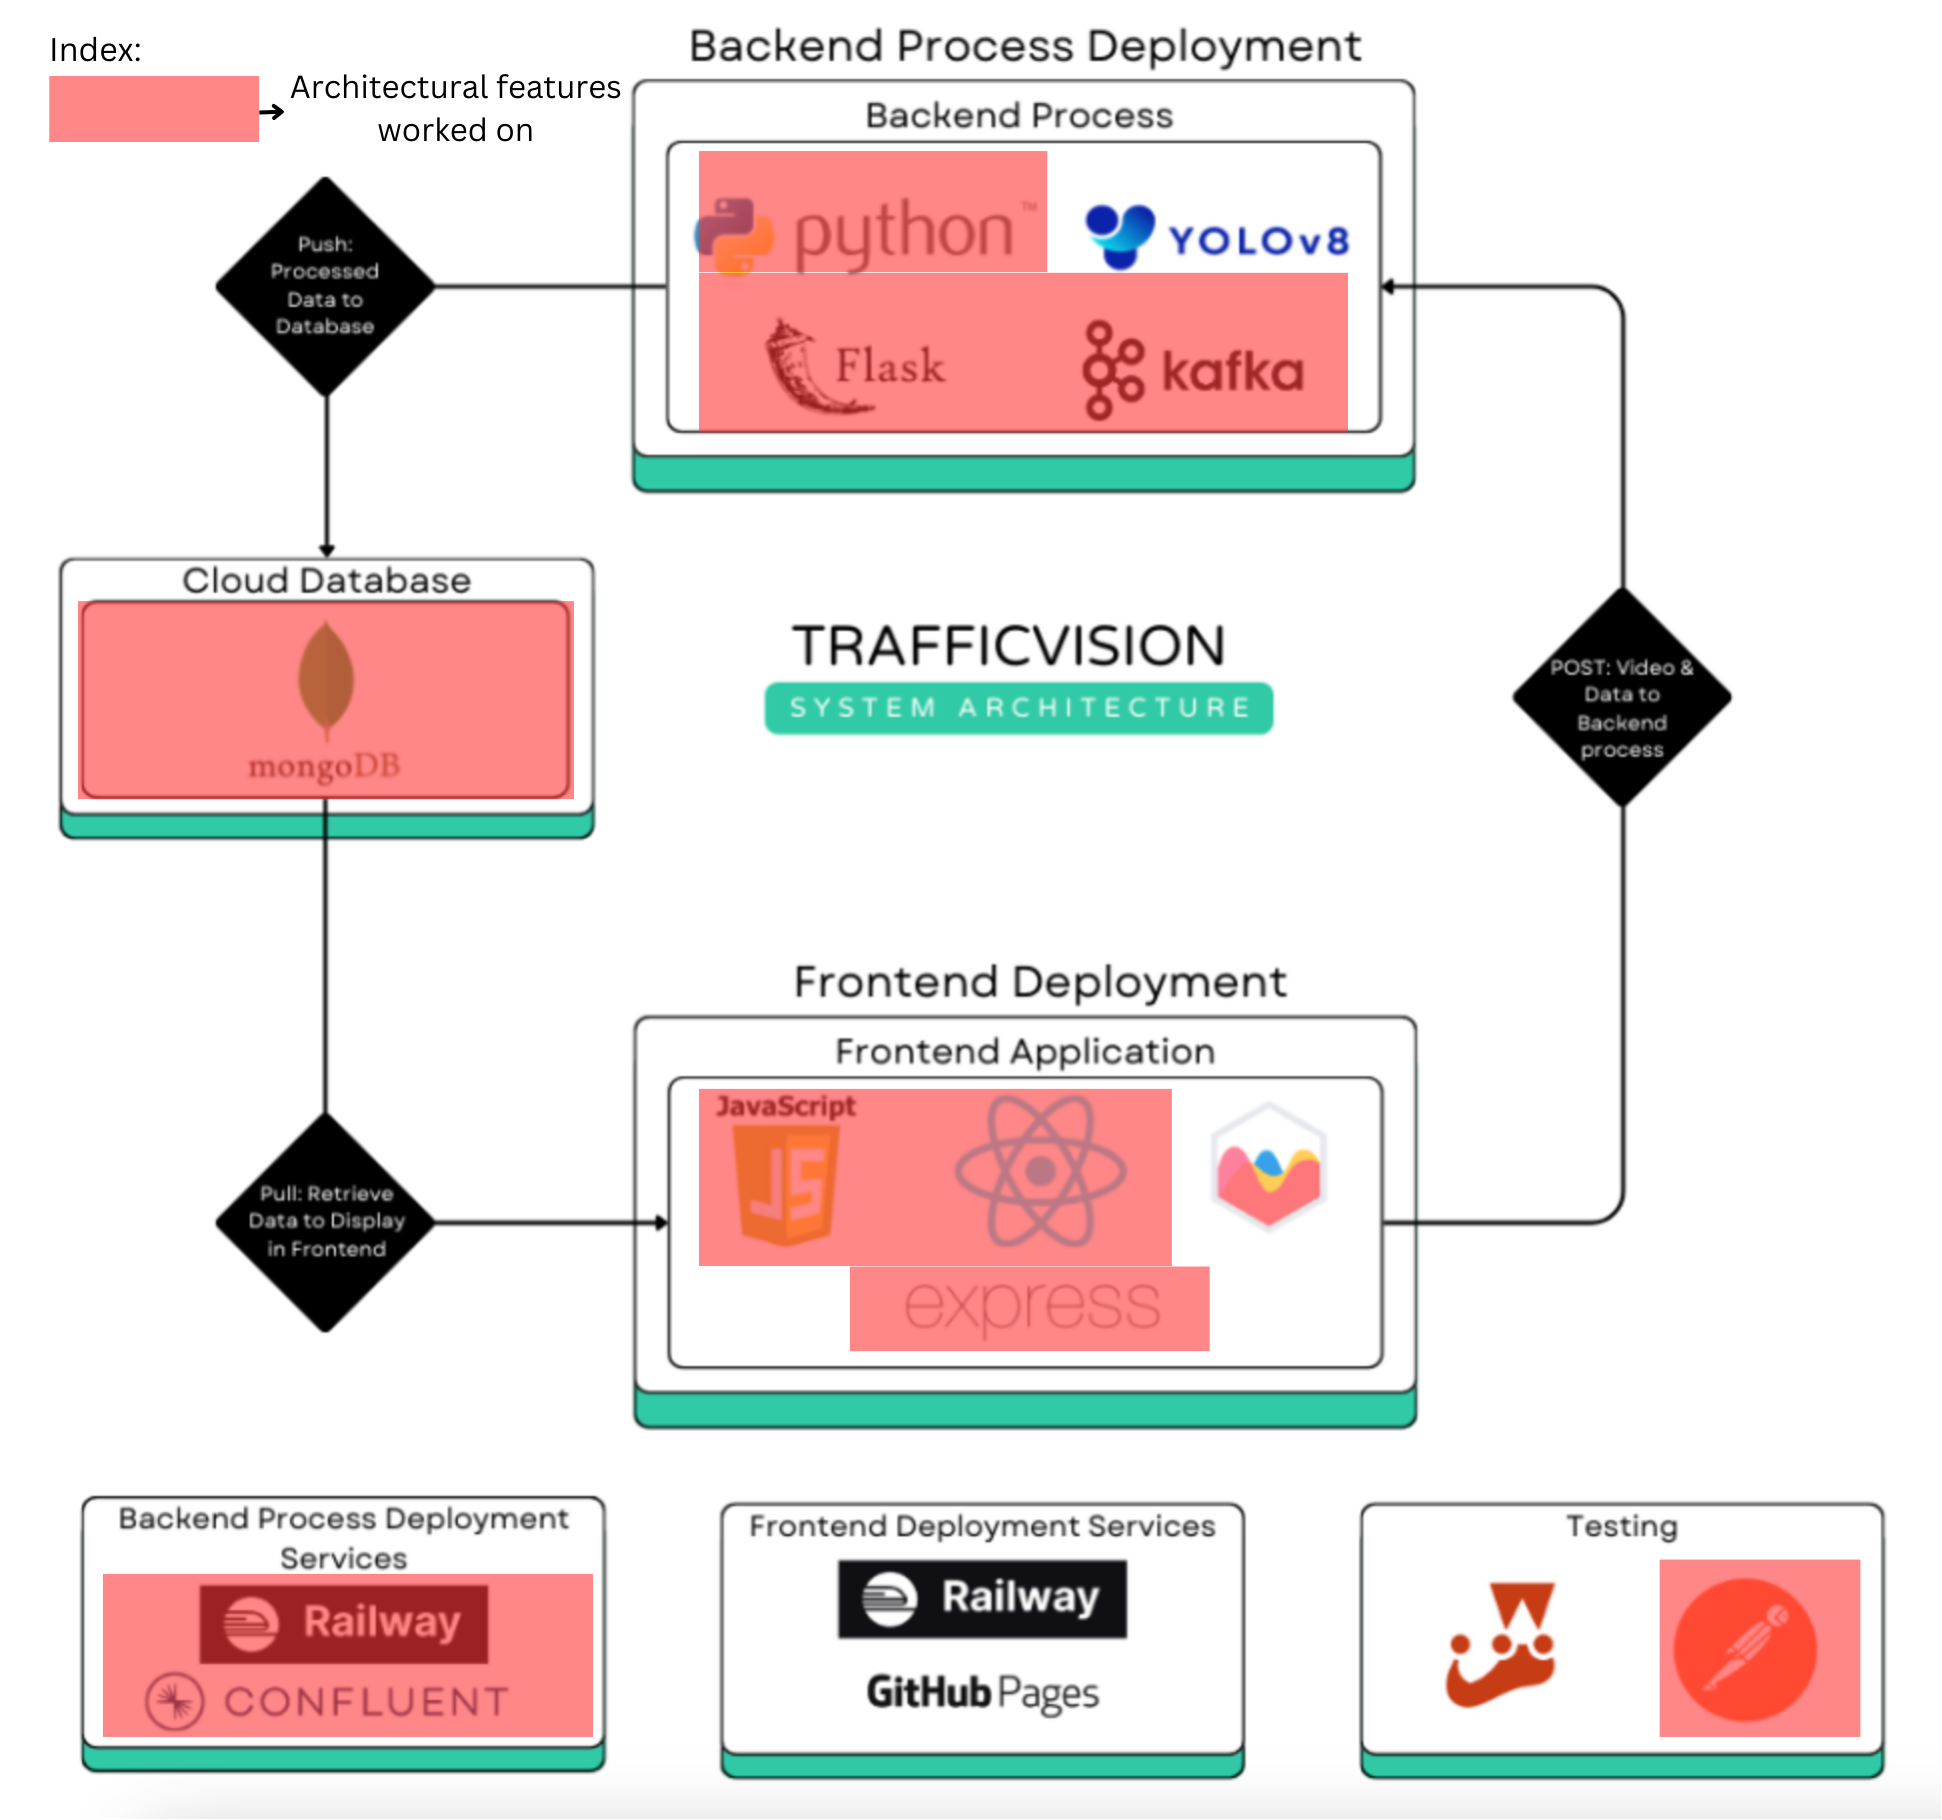
\includegraphics[width=0.9\textwidth]{images/architecture.png}
    \caption{System Architecture.}
    \label{image:sysArchitecture}
\end{figure}

\begin{figure}[H]
    \centering
    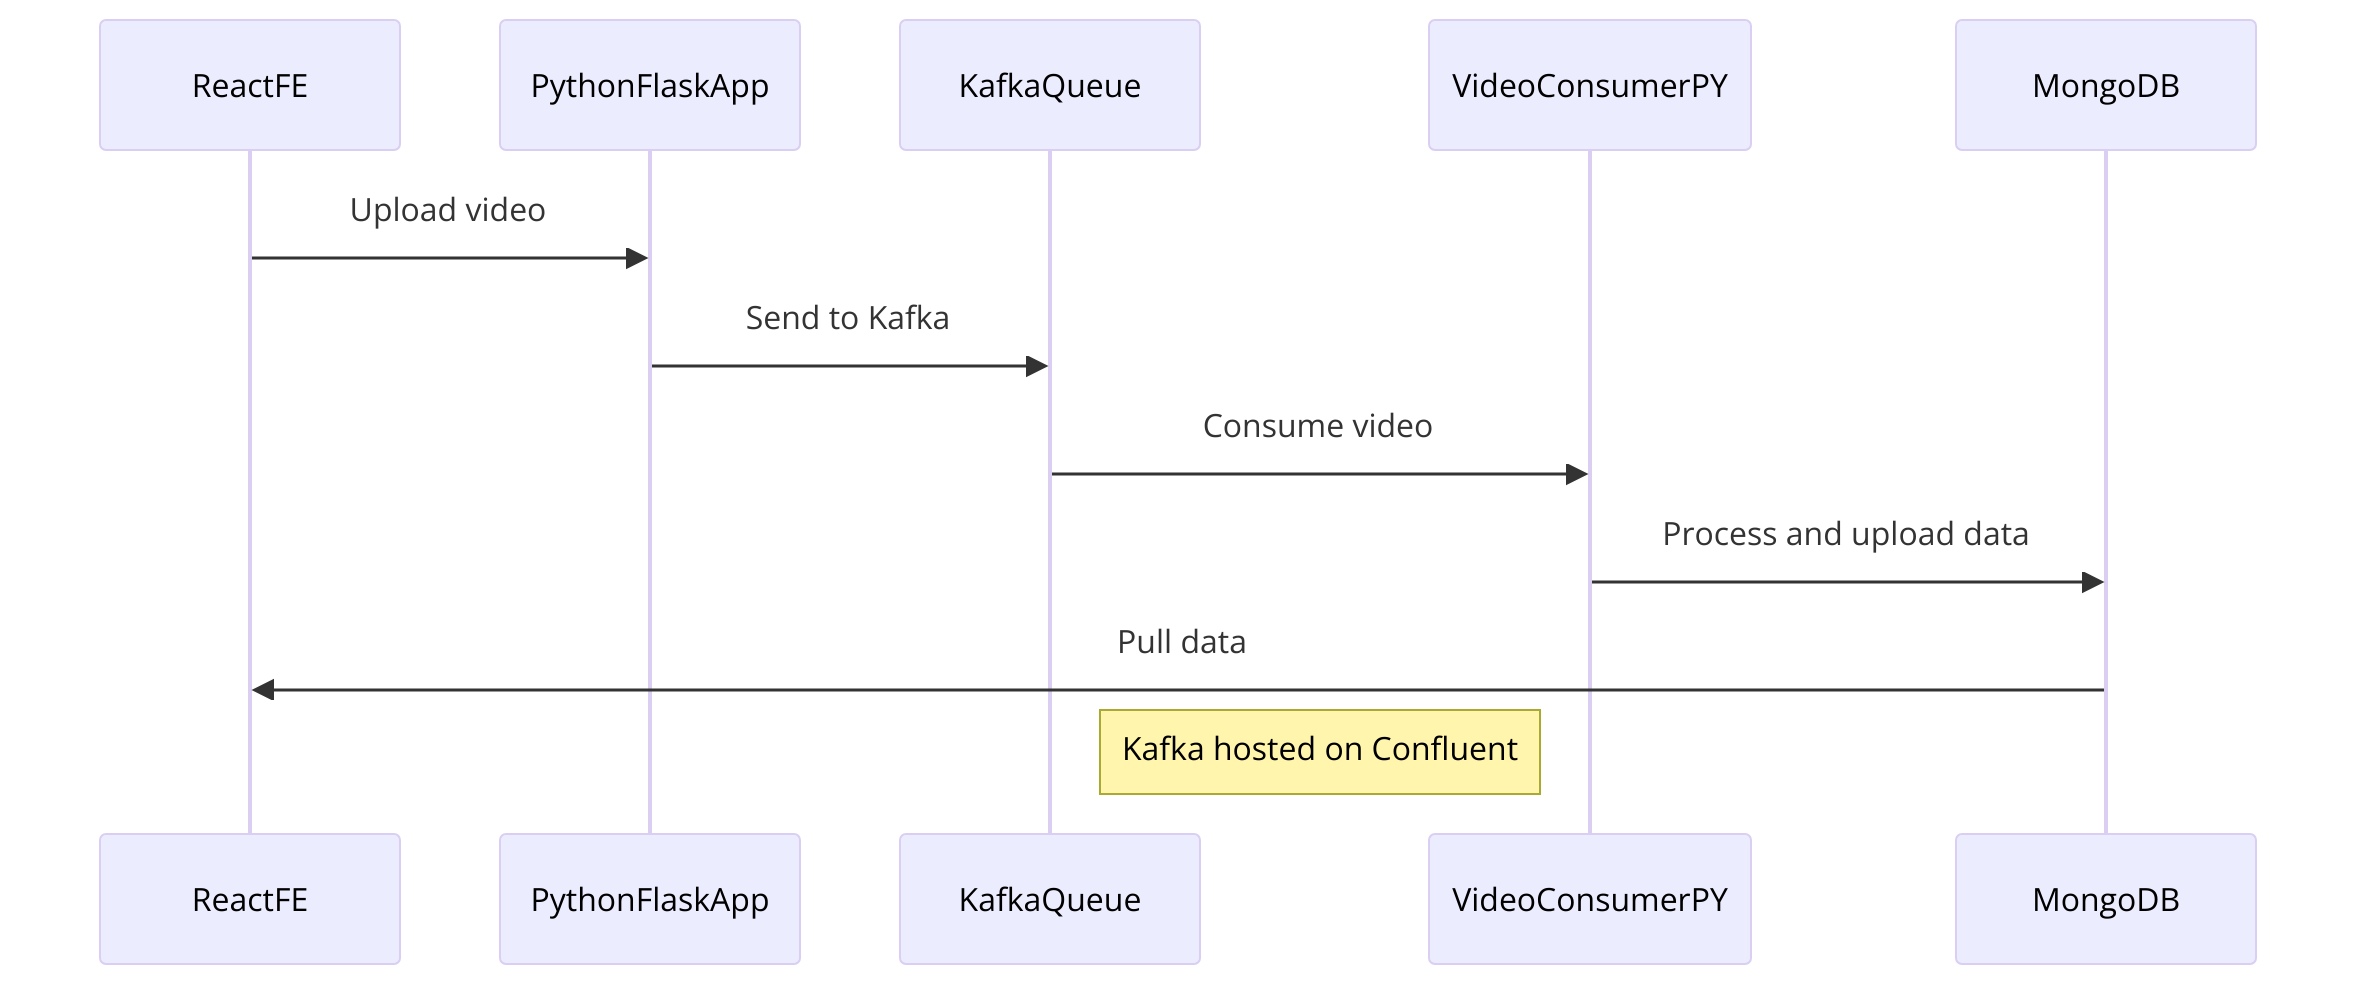
\includegraphics[width=0.9\textwidth]{images/systemFlowChart.png}
    \caption{Flowchart\cite{lucidchartDataFlow} of TrafficVision System Operations.}
    \label{fig:systemFlowChart}
\end{figure}


\section{TrafficVision System Architecture}

\subsection{Frontend Deployment}
The frontend of TrafficVision is constructed using React, a  JavaScript library for building user interfaces. The choice of React is attributed to its component-based architecture, which facilitates the development of interactive UIs.
\begin{itemize}
    \item Users use this frontend to upload traffic videos and additional data into the system, initiating the data processing workflow.
\end{itemize}

\subsection{Serverless Deployment: Processing Server}
Upon user interaction with the frontend, video and data uploads trigger actions within a serverless processing server.
\begin{itemize}
    \item The serverless model, functioning as a function-as-a-service (FaaS), dynamically executes backend code in response to events, in this scenario, video uploads, circumventing the need for a persistent server environment.
    
    \item The processing server operates on a Python runtime, renowned for its extensive libraries that support a multitude of web and data processing functionalities.
    
    \item Within this server, two technologies are utilized:
    \begin{itemize}
        \item \textbf{YOLOv8 (You Only Look Once):} This state-of-the-art deep learning algorithm specializes in object detection within video frames in real-time, identifying vehicles and other objects promptly and accurately.
        
        \item \textbf{Apache Kafka:} A robust distributed event streaming platform that orchestrates real-time data feeds. Kafka manages the flow of data throughout the system components, particularly by queuing video processing tasks efficiently.
    \end{itemize}
\end{itemize}

\subsection{Cloud Database: MongoDB}
Post-processing of video data, MongoDB, a NoSQL cloud database, is employed to manage the data output.
\begin{itemize}
    \item MongoDB is chosen for its adaptable, schema-less data structure and powerful scalability, which is ideal for handling the vast and varied datasets of TrafficVision.
    
    \item The database serves as a repository for processed traffic data, which can be later fetched by the frontend for display and analysis purposes.
\end{itemize}

\subsection{Kafka Deployment on Confluent}
Apache Kafka's deployment within the TrafficVision system is facilitated through Confluent, which is a fully managed Kafka service that simplifies the process of running Kafka.

The following snippet of code simplifies the Kafka configuration for connecting to the Confluent service:

\begin{verbatim}
kafka_config = {
    "bootstrap.servers": os.getenv("KAFKA_BROKER_URL"),
    "security.protocol": "SASL_SSL",
    "sasl.mechanisms": "PLAIN",
    "sasl.username": os.getenv("KAFKA_API_KEY"),
    "sasl.password": os.getenv("KAFKA_API_SECRET"), 
    ...
}
\end{verbatim}

This configuration uses the Producer and Consumer components ensuring they communicate efficiently with the Kafka cluster hosted on Confluent. The TrafficVision system uses Confluent's managed Kafka solution to ensure high-throughput data processing and streamlining the real-time video analytics pipeline.

\subsection{Data Flow}
The operation of TrafficVision encompasses a series of coordinated processes:
\begin{itemize}
    \item \textbf{Video Upload:} Utilizing the frontend application, users upload videos to the processing server, instigating an event that forwards the video and associated data to the server for processing.
    
    \item \textbf{Data Processing:} Leveraging serverless deployment, video data is processed in real-time. Kafka's queuing system allows for scalable and parallel processing of multiple video streams.
    
    \item \textbf{Data Storage:} Upon processing the data is stored in MongoDB, making it accessible for subsequent retrieval.
    
    \item \textbf{Data Retrieval:} The React-based frontend retrieves processed video data from MongoDB, presenting users with comprehensive traffic analysis and insights.
\end{itemize}

\begin{figure}[H]
    \centering
    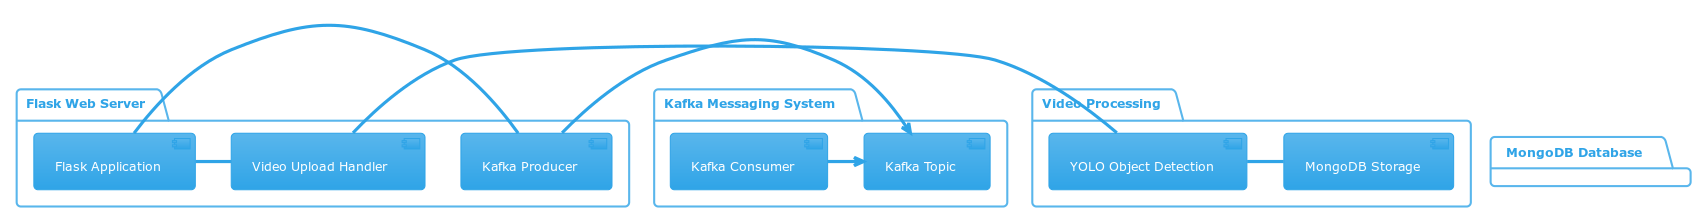
\includegraphics[width=0.9\textwidth]{images/mapDiagram.png}
    \caption{Map Diagram of the TrafficVision Data Flow.}
    \label{fig:mapDiagram}
\end{figure}


\section{Component Interaction and Code Correlation}

The TrafficVision system's UML\cite{umlDiagramMiro} diagram provides a detailed overview of the component interactions within the architecture. The diagram is essential in understanding the system's modularity and connectivity between components.

\subsection{Flask Application}

The \texttt{FlaskApplication} acts as the interface for client interactions. It handles HTTP requests including video uploads and assigns tasks to other components. The following code snippet represents the video upload handling within the Flask application, corresponding to the \texttt{route} method in the UML class:

\begin{verbatim}
@app.route("/upload", methods=["POST"])
def upload_video():
    # [Code to handle video upload]
\end{verbatim}

\subsection{Kafka Producer}

The \texttt{Producer} sends messages to the Kafka cluster. Upon a successful video upload the producer sends a message containing the video ID and metadata, as shown in the code below:

\begin{verbatim}
try:
    producer.produce("incoming-videos", key=str(uuid.uuid4()), value=message)
    producer.flush()
except Exception as e:
    # [Error handling code]
\end{verbatim}

\subsection{YOLO Object Detection}

The \texttt{YOLO} class represents the object detection component using the YOLOv8 algorithm. The code snippet below shows the model loading and video processing, which correlates with the UML diagram:

\begin{verbatim}
model = YOLO("yolov8n.pt")
# [Code to process video and detect objects]
\end{verbatim}

\subsection{MongoDB Storage}

The \texttt{MongoClient} handles data storage in MongoDB. The process of inserting data into the database is represented in the following snippet:

\begin{verbatim}
if info_list:
    collection.insert_many(info_list)
    # [Code to handle database insertion]
\end{verbatim}

\subsection{Integration and Workflow}

Integrating these components allows for a seamless flow from video upload to object detection and data storage. The provided code offers a concrete implementation of the conceptual UML structure.

\begin{figure}[H]
    \centering
    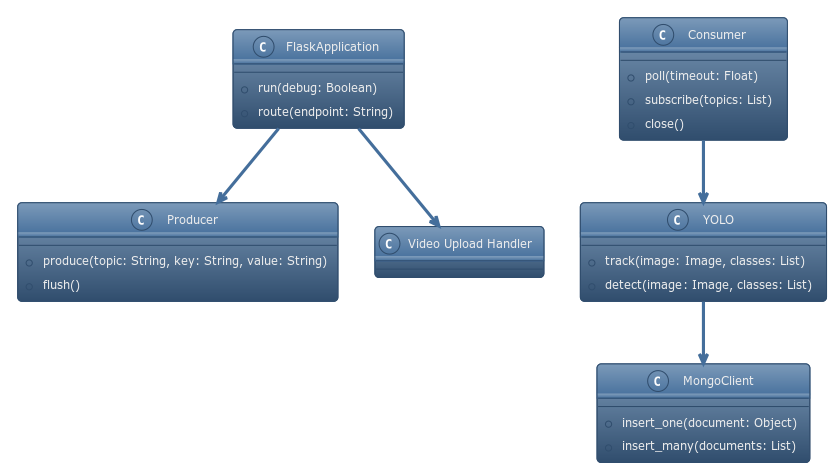
\includegraphics[width=0.9\textwidth]{images/uml.png}
    \caption{UML Diagram of TrafficVision Components.}
    \label{fig:umlDiagram}
\end{figure}

This UML diagram showcases the individual responsibilities of each system component and its modularity within TrafficVision for efficient traffic video processing and analysis.


\section{Environment Configuration with \texttt{.env} Files}

\subsection{Purpose and Benefits}

The TrafficVision system uses \texttt{.env}\cite{gentleIntroductionEnvFiles} files to manage environment variables, which are crucial for defining the runtime environment configuration outside of the codebase. This approach separates configuration from code, which is a principle of a twelve-factor app methodology\cite{twelveFactor} leading to several advantages:

\begin{itemize}
    \item \textbf{Security:} Sensitive information such as API keys and database credentials are kept out of the version control system reducing the risk of security breaches.
    \item \textbf{Portability:} Developers can create multiple \texttt{.env} files for different environments like development, testing and production making it easier to manage and deploy the application across various environments.
    \item \textbf{Customization:} Each instance of the application can be easily customized by changing the environment variables without altering the code.
\end{itemize}

\subsection{Implementation in TrafficVision}

The TrafficVision system utilizes the \texttt{dotenv} library for Python to load the configuration variables from the \texttt{.env} file when the application starts. The following code snippet shows how the environment variables are loaded:

\begin{verbatim}
from dotenv import load_dotenv
DOTENV_PATH = "./.env"
load_dotenv(dotenv_path=DOTENV_PATH)
\end{verbatim}

This simple yet effective setup allows the application to access the environment variables as needed, for instance:

\begin{verbatim}
kafka_config = {
    "bootstrap.servers": os.getenv("KAFKA_BROKER_URL"),
    ...
    "sasl.password": os.getenv("KAFKA_API_SECRET"),
}
\end{verbatim}

In this example the Kafka connection configuration is built using values sourced from the environment which allows for flexibility and security.

\subsection{Implication}
TrafficVision's system design utilizes cutting edge technologies and practices to make a flexible and effective traffic management solution. Front and center of its frontend is React's user friendly user interface, where traffic information can be uploaded. This user interaction launches a backend response in the backend which handles video data uploads dynamically.

YOLOv8's real time object detection and Apache Kafka's information streaming are central to the system processing abilities, all hosted in the scalable Confluent managed services environment. These technologies work together to provide quick and precise processing of traffic videos, queuing activities and smartly managing information flows.

Persistence and results of processed information are handled by MongoDB, a NoSQL cloud database with adaptable data structure and scalability which successfully handles the different produced data sets.

TrafficVision's environment configuration approach based on.env documents highlights the system's operational flexibility and security. By externalizing configuration detail, TrafficVision secures very sensitive information and offers flexibility to adapt to various deployment environments without refactoring the core codebase.

To sum up, TrafficVision's system architecture is a mix of intuitive user interfaces, serverless backend computing, information processing, and configuration management security. This sophisticated integration allows TrafficVision to offer effective traffic analysis.
\chapter{System Evaluation}
This chapter evaluates the TrafficVision project against the objectives set out in the introduction. Here presenting the results obtained from the system's operation and discuss its strengths and weaknesses. This evaluation serves as a platform to demonstrate critical thinking in relation to the project and its outcomes.

\section{Objective Alignment}
The primary objectives of TrafficVision were to provide real-time traffic monitoring, enhance public transportation system reliability and improve user engagement through interactive features. The following sections detail how the system has met these objectives and highlight areas for further development.

\section{Real-Time Traffic Monitoring}
One of TrafficVision's core objectives was to implement real-time traffic monitoring. The system's ability to process and display live traffic conditions is illustrated in Figure \ref{fig:videoProcessing}.

\begin{figure}[H]
    \centering
    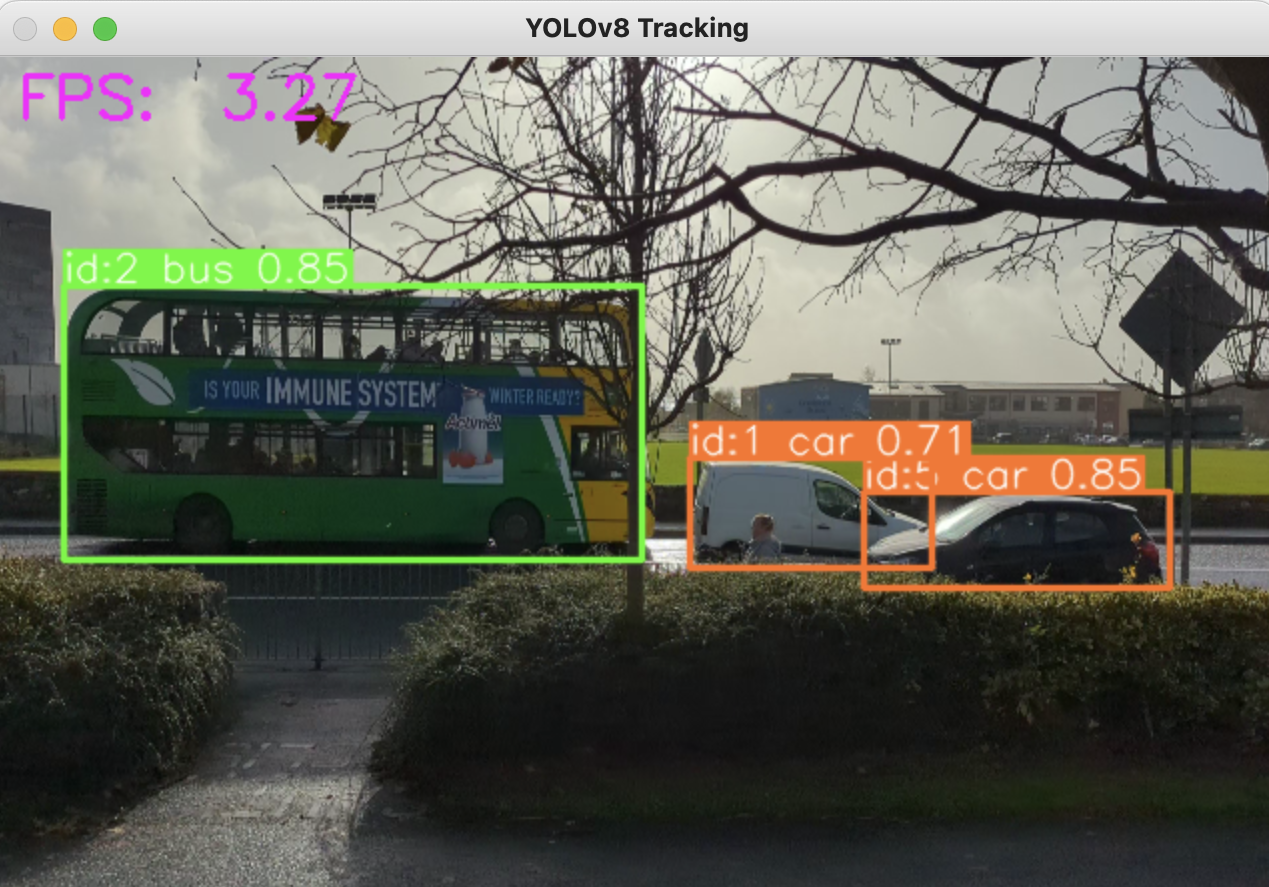
\includegraphics[width=1\linewidth]{images/videoProcessing.png}
    \caption{TrafficVision's real-time traffic monitoring interface demonstrating vehicle detection and tracking.}
    \label{fig:videoProcessing}
\end{figure}

The system successfully identifies and tracks vehicles with high accuracy and low latency, as shown in the terminal outputs in Figure \ref{fig:pythonTerminal}. However, one weakness observed is the dependency on good lighting conditions for optimal performance, which could be addressed with enhanced image preprocessing techniques or the integration of infrared camera feeds for night-time monitoring.  Future enhancements for the TrafficVision real-time monitoring system may include the integration of additional data sources such as traffic cameras across different locations, which would provide a more comprehensive traffic analysis. Additionally, machine learning techniques could be employed to predict traffic conditions based on historical data, providing users with not only the current state of traffic but also an intelligent forecast of short-term changes.

\begin{figure}[H]
    \centering
    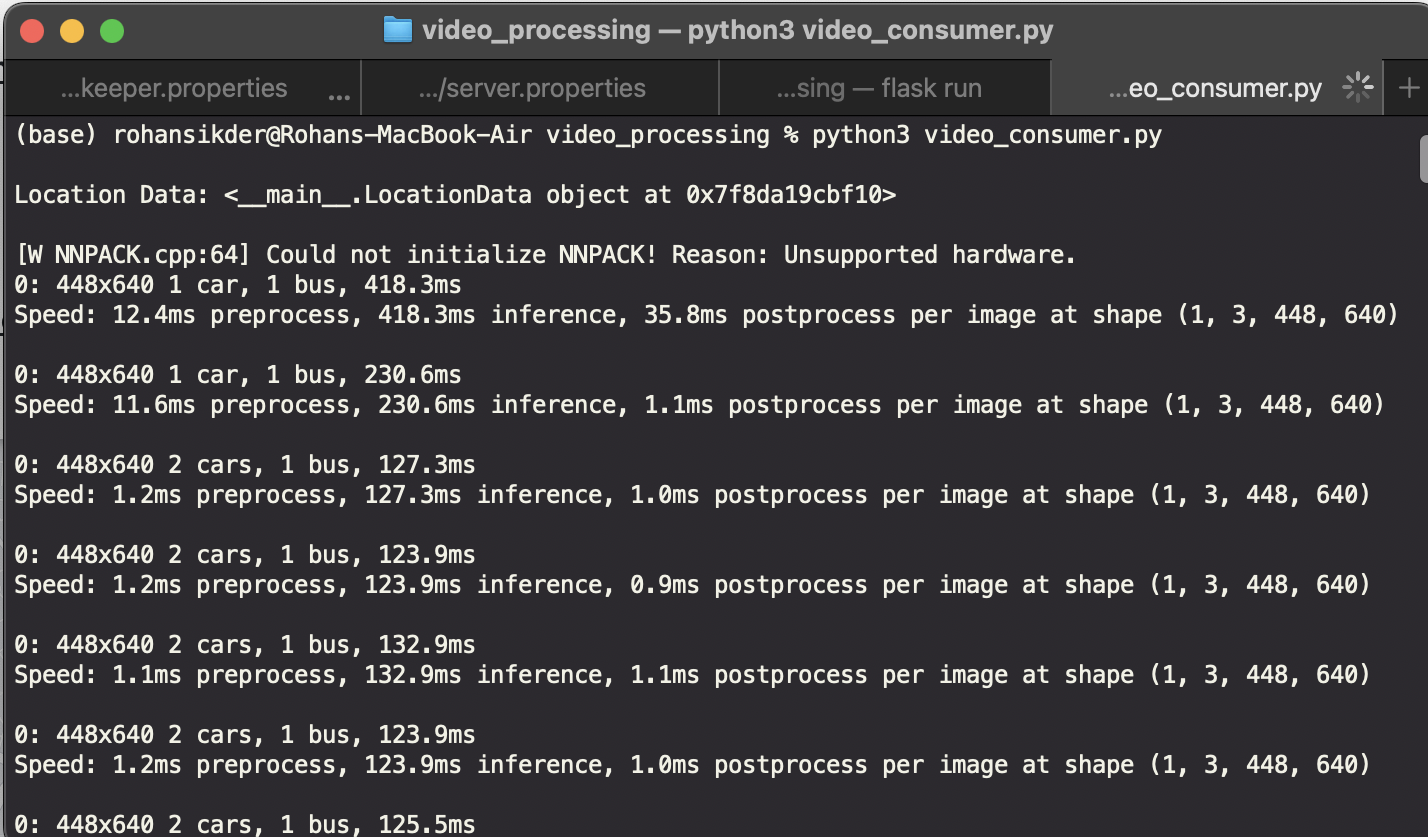
\includegraphics[width=1\linewidth]{images/pythonTerminal.png}
    \caption{Performance metrics of the TrafficVision system captured from the terminal output.}
    \label{fig:pythonTerminal}
\end{figure}

\section{Public Transportation System Reliability}

Enhancing the reliability of public transportation was another key objective. TrafficVision contributes to this by analyzing bus punctuality, as depicted in Figure \ref{fig:busUI}. The graph shows the frequency of bus appearances and can be used to assess punctuality against the schedule.

\begin{figure}[H]
    \centering
    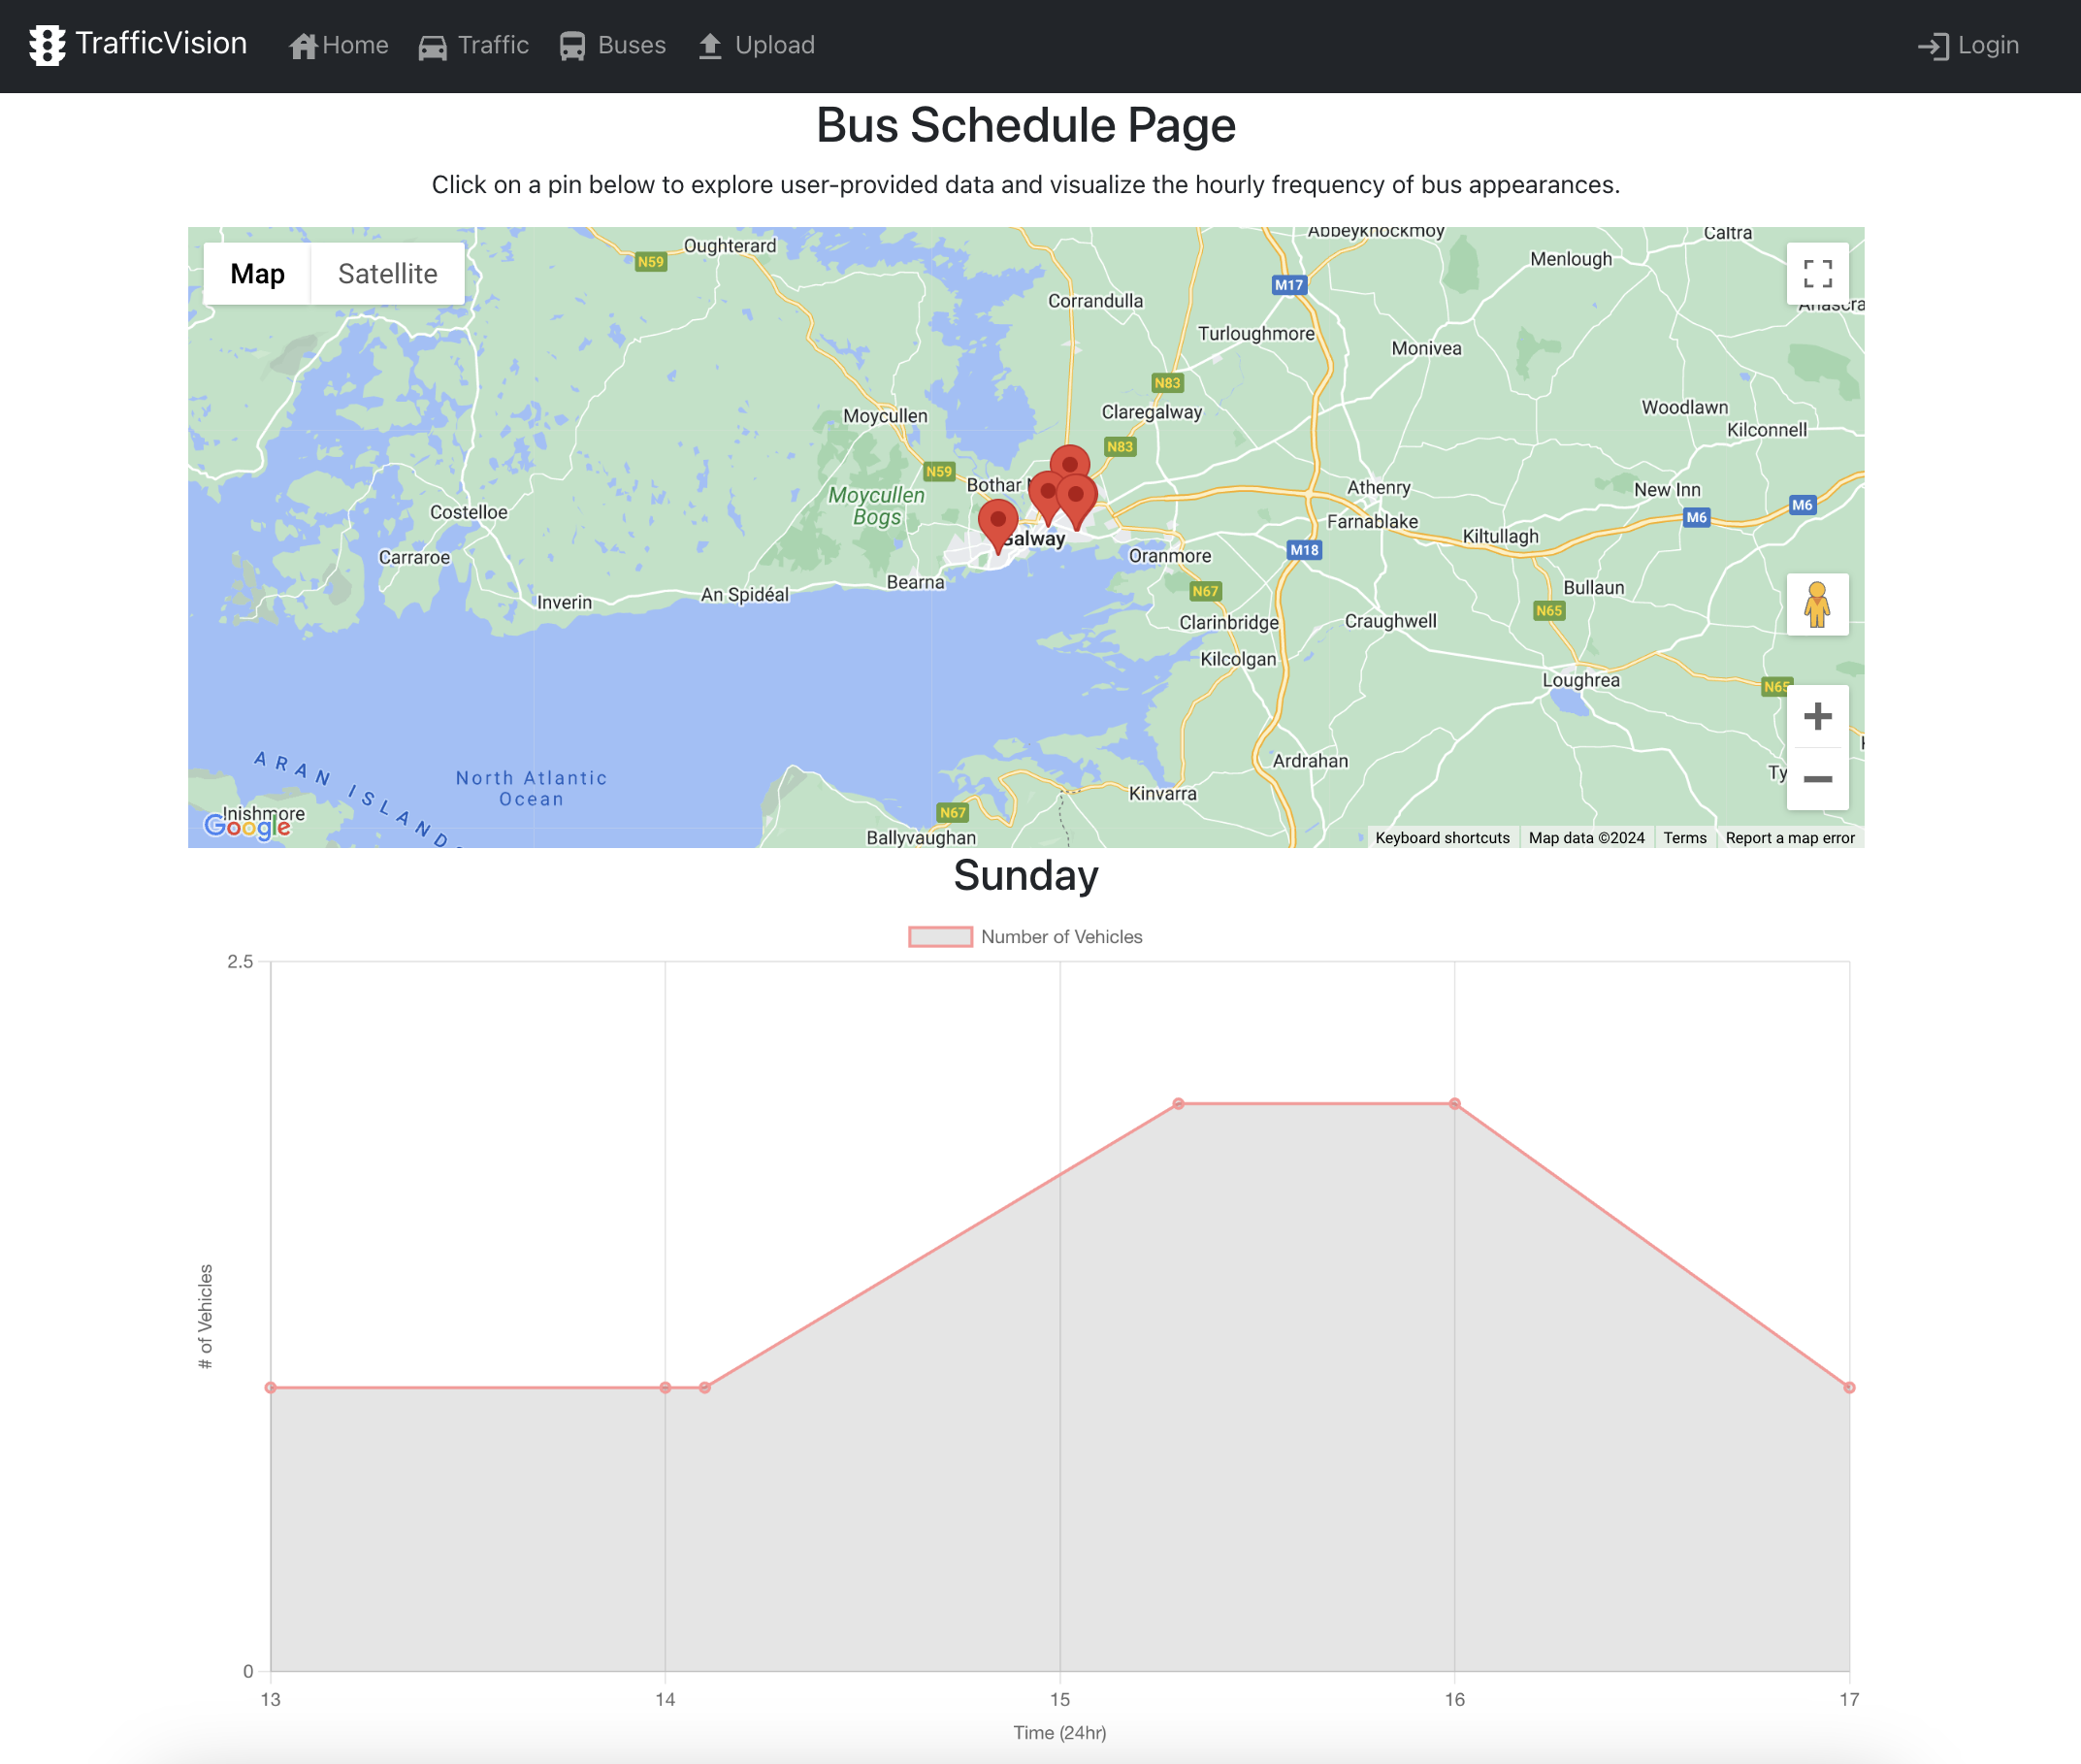
\includegraphics[width=\linewidth]{images/busUI.png}
    \caption{Visualization of bus schedule adherence using TrafficVision's data analytics.}
    \label{fig:busUI}
\end{figure}

While the system effectively records bus frequencies, the strength of the data is dependent on the quantity and quality of user submissions. This represents a limitation in data collection that could potentially be overcome with more widespread user participation or the incorporation of official transit data feeds.

\section{Integration Challenges with Transport for Ireland API}
The implementation of the Transport for Ireland API into the TrafficVision system was not a option due to the lack of documentation and complexity of the API. The API, which provides real-time bus schedules with arrival and departure times, was critical to compare how late buses were.

After research on attempts to integrate this API due to the significant challenges faced, including the API being oriented towards internal use by Transport for Ireland. Restricted accessibility making it not suitable for the TrafficVision project.

Alternative data sources were looked at that could provide accurate real time bus schedules along with departure and arrival times. However, no suitable alternatives were identified that satisfied the project's specific accessibility, reliability and integration needs.

\section{User Engagement and Interaction}

User engagement is critical for crowd-sourced platforms like TrafficVision. The UI and UX are designed to be intuitive and engaging, as evident in the system's login page (Figure \ref{fig:loginUI}) and the traffic upload feature (Figure \ref{fig:uploadUI}).

\begin{figure}[H]
    \centering
    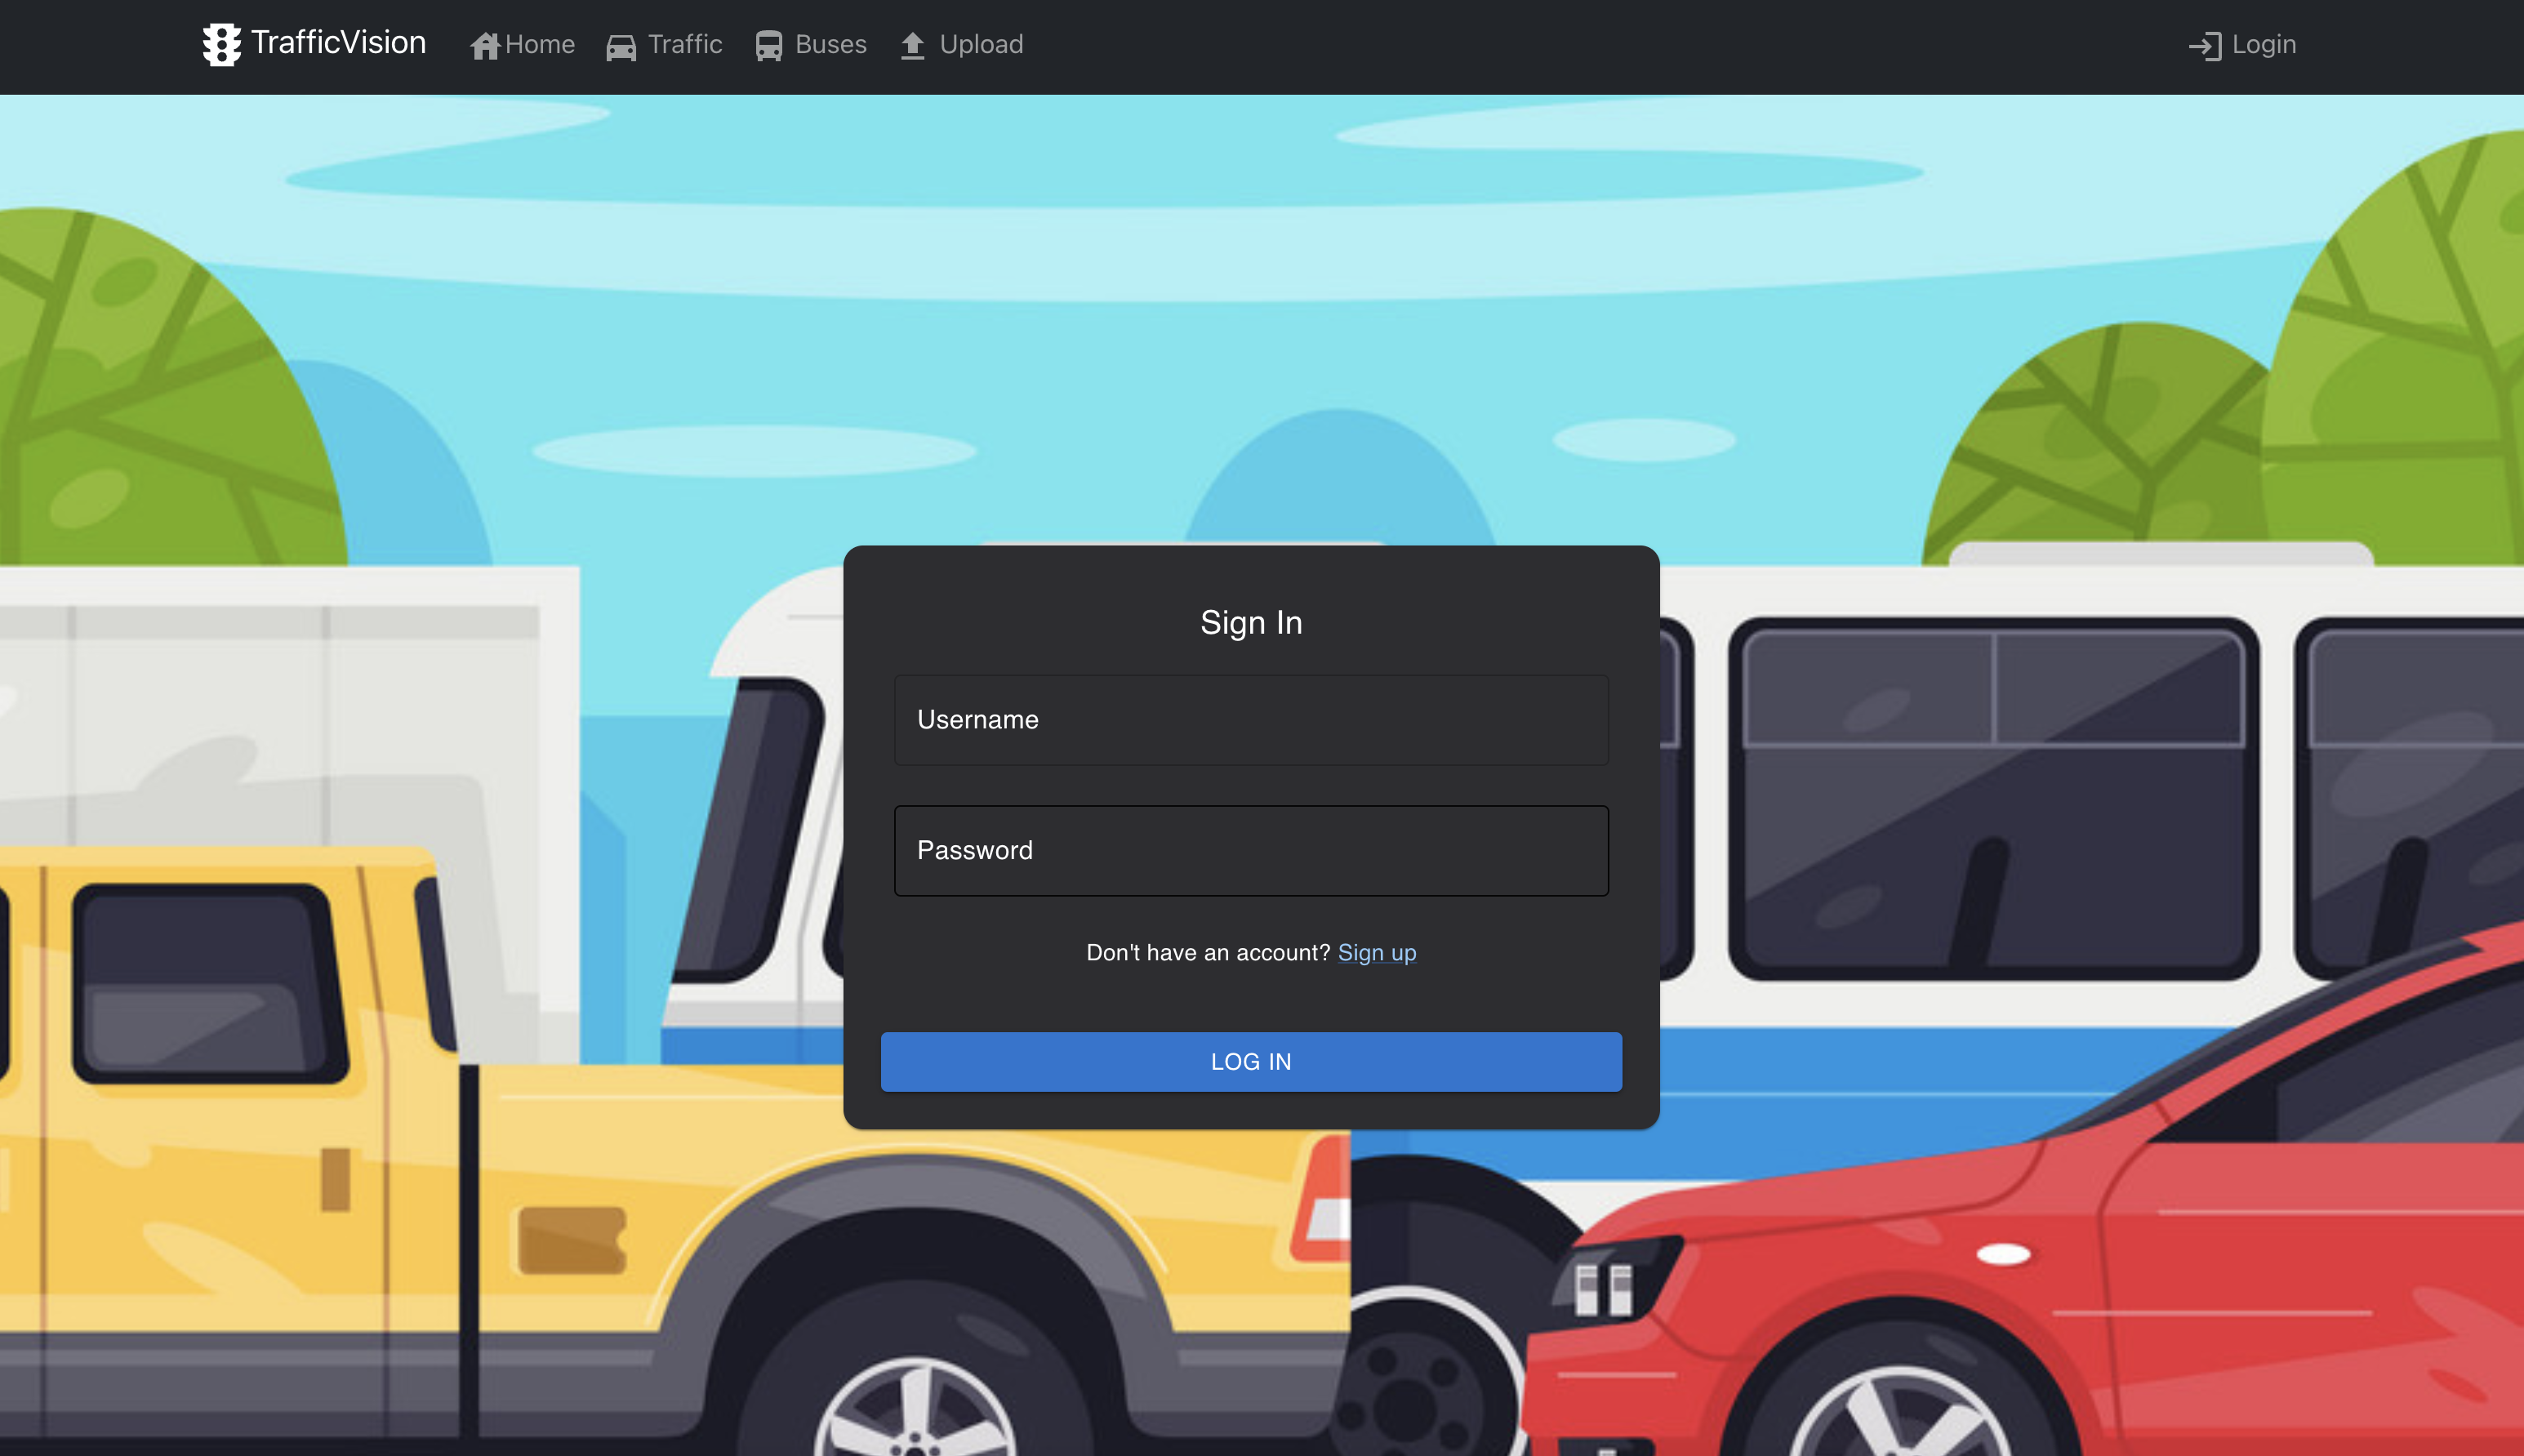
\includegraphics[width=\linewidth]{images/loginUI.png}
    \caption{The login page of TrafficVision, showcasing the system's user-friendly interface.}
    \label{fig:loginUI}
\end{figure}

\begin{figure}[H]
    \centering
    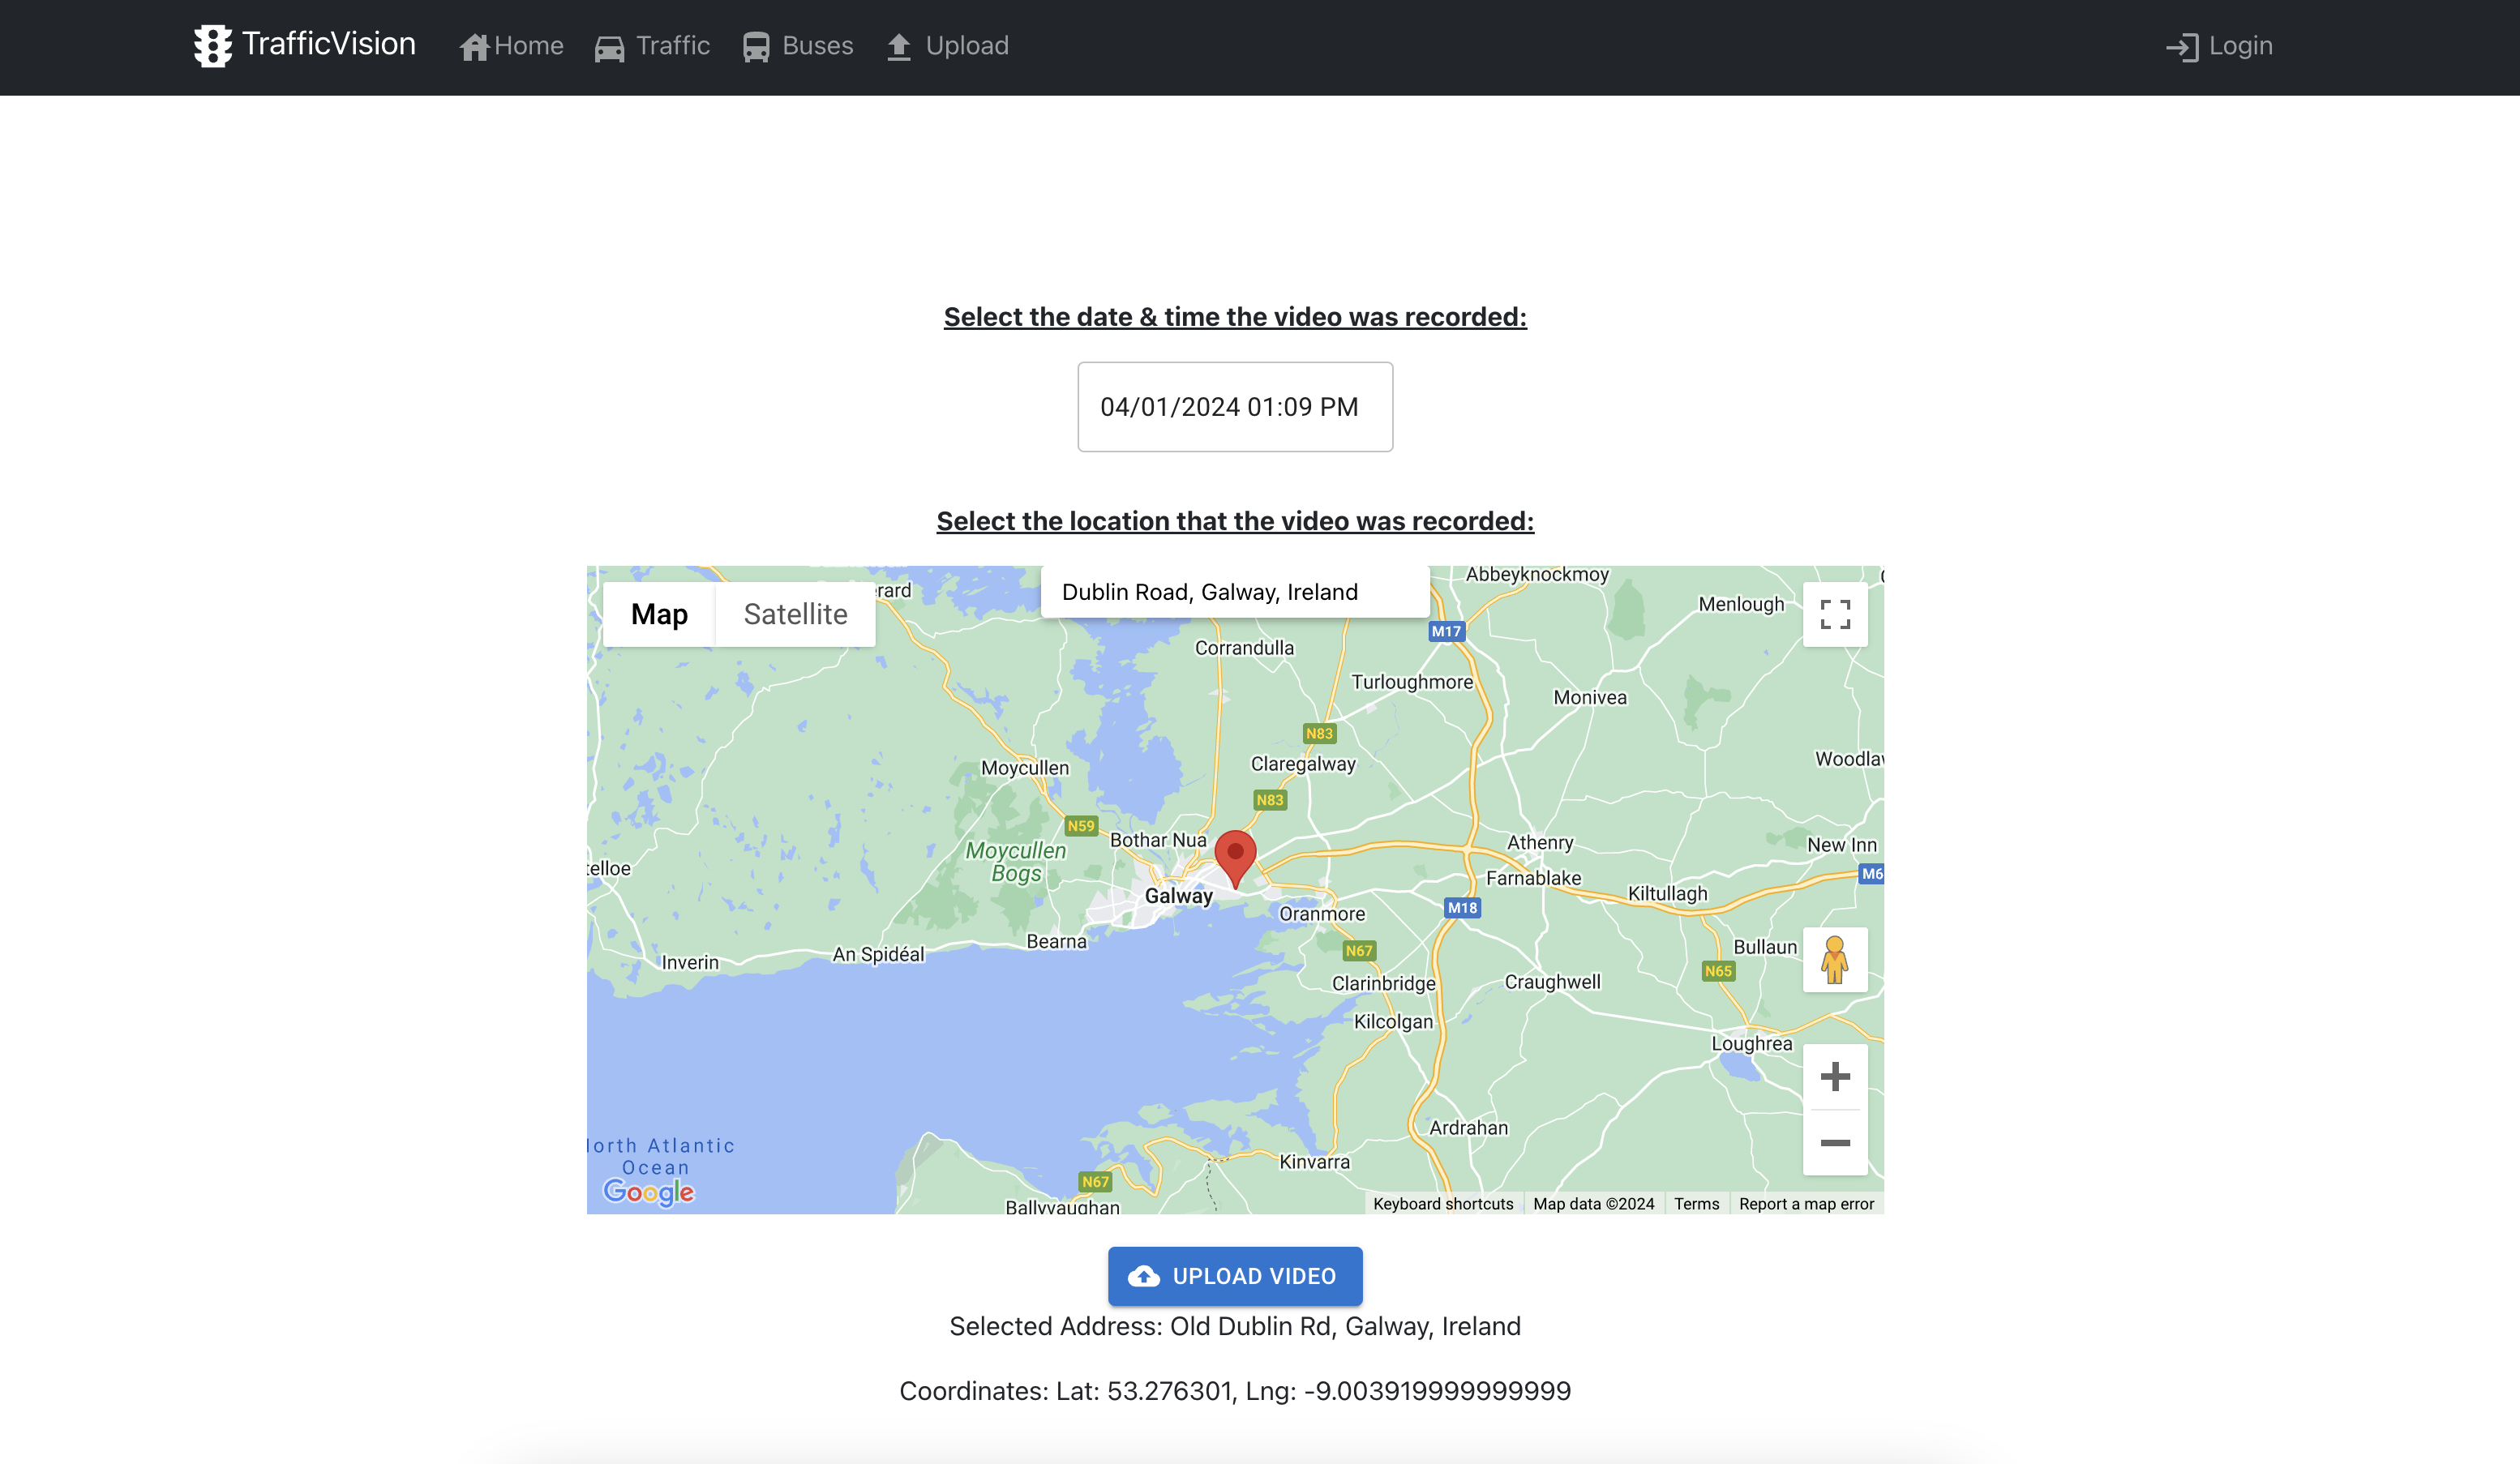
\includegraphics[width=\linewidth]{images/uploadUI.png}
    \caption{TrafficVision's video upload feature, enabling user participation in traffic data crowdsourcing.}
    \label{fig:uploadUI}
\end{figure}

While the system provides a straightforward mechanism for users to contribute data, a notable weakness is the reliance on active user engagement, which may lead to data sparsity. Future enhancements could include gamification elements to incentivize regular contributions or the use of passive data collection methods.

\section{Deployment Challenges}
The TrafficVision system deployment presented significant technical challenges, especially in handling the large scale video processing requirements. The initial deployment strategy used cloud services like AWS which provided extensive resources but had cost and scalability issues due to traffic volumes fluctuating.

To address these concerns, the project shifted toward using Railway\cite{railway2024}, a platform that supports Docker, aiming to simplify the deployment process through containerization. This way we could have a more manageable configuration of our Python applications and dependency management.

Given challenges the challenges met in researching and developing a deployment, the most effective deployment of the TrafficVision system has been on local machines, where video processing can be managed more reliably.

In the future, optimization of the deployment architecture will be a priority, such as stronger cloud offerings or dedicated hardware to handle high video processing. This includes testing machine learning models optimized for resource efficiency and integrating adaptive streaming technologies.

\section{Cross-Platform Development Challenges}
A small team of two members worked on TrafficVision using two different operating systems: Unix and Windows. This configuration introduced special system compatibility and integration issues when using technologies like Confluent for Kafka streams, MongoDB for database management and Python for backend and video processing.

These compatibility issues highlighted the need for development practices that support both environments. The team considered several ways to coordinate their development efforts including:

\begin{itemize}
    \item \textbf{Standardization of Development Tools:} The team focused on using cross-platform compatible tools and technologies to reduce system incompatibility issues. This approach was vital to ensure that all components of the TrafficVision system worked harmoniously across different operating environments.
    \item \textbf{Version Control Systems:} Strong version control practices became critical for effective change management and maintaining system stability across different operating systems. By employing robust version control, the team could manage code changes more efficiently, ensuring that updates did not disrupt the system's operation on any platform.
\end{itemize}

In the future, the team sees the potential in virtual environments integrating into their workflow. Future projects using virtual environments could deliver better development efficiency due to the consistent development settings across systems. This would simplify the development cycle, cut down setup time and reduce compatibility issues.

This experience helped to understand how to work together in a mixed system context, preparing the team for future work involving different development platforms.

\section{Strengths and Weaknesses Summary}
The evaluation of TrafficVision against the set objectives has demonstrated strengths in real-time processing, user interface design and traffic data visualization. Weaknesses are mainly centered around data dependence on user engagement and environmental conditions affecting data acquisition. Addressing these weaknesses will be crucial for the next phase of development, focusing on system robustness and data diversity.

Overall, TrafficVision has made significant strides toward its envisioned goals, laying a solid foundation for future enhancements in traffic monitoring and analysis.
\chapter{Conclusion}
This dissertation has explored the development and deployment of TrafficVision, a web application that aims to transform urban mobility through real time traffic monitoring and advanced analytics. The main focus of this large scale project was to improve the network reliability of public transport services, commuter wait times and sustainable urbanization through traffic congestion and emissions reduction.

TrafficVision was developed using OpenCV for video processing, YOLOv8 for object detection, Kafka for data handling and MongoDB for data storage. These technologies were combined to process real-time video data. Database management systems was crucial for analyzing urban traffic patterns and improving public transport reliability and punctuality.

On a closer look, TrafficVision was a success in achieving its initial goals due to its real-time traffic status reports and bus schedule compliance. This critical feature allows commuters and urban planners to make informed decisions that significantly improved commuting efficiency and traffic control. However, TrafficVision currently has a limit on the amount of crowdsourced data it processes. With more data collection the system will become more precise and useful in terms of deep insights and more accurate traffic forecasts.

One of TrafficVision's key functions is providing transportation authorities and government entities with real-time information about bus punctuality and traffic density. This info is clear evidence that could be used to lobby for required reforms in the public transport system. TrafficVision identifies bus service problem areas and peak times with high delays and supports targeted interventions to reduce traffic congestion and improve bus service efficiency.

\subsection{Future improvements}
Future improvements to TrafficVision are numerous. Future developments could mainly focus on extending data collection techniques to cover more passive data streams and on enhancing system robustness to various environmental conditions. High-end image processing technologies could be combined to work well in different lighting and weather conditions to achieve uniform performance regardless of external conditions.

Furthermore, collaboration with local governments and transportation authorities could enhance data quality and comprehensiveness and extend TrafficVision's reach across geographic and operational boundaries. Such collaborations could also enable TrafficVision to be incorporated into official traffic management and urban planning initiatives as a core technology for smart city initiatives.

TrafficVision provided a solid foundation for the future of traffic management systems and demonstrated the potential of technology in resolving challenging urban mobility issues. The user-contributed data will continue to refine TrafficVision as a useful tool for urban planning and public transportation optimization. With ongoing technological developments and enhanced user engagement, TrafficVision will be considered a key element of future smart cities and will lead to transformation of public transportation.

\subsection{In conclusion}
TrafficVision met its initial objectives of proving it was capable of boosting the public transportation reliability via real time traffic monitoring. However with increased time for deployment and a bigger dataset the application would have further refined during its first functional stage. These enhancements would refine the system's accuracy and user interface, setting the foundation for its subsequent development stages.

Looking forward, machine learning could be used to analyze the massive traffic data collected. This advancement will enable TrafficVision to not just react to actual traffic situations but also predict the real traffic patterns to better inform urbanized transportation methods. Such predictive features, coupled with environmental traffic monitoring (like emissions monitoring),would expand TrafficVision into a more of a tool for city planning and sustainability.

\appendix
\chapter{Project Resources}
\label{appendix:resources}

\begin{itemize}
    \item Video Demo: \href{https://github.com/ConorPadraigMurphy/FYP/blob/main/RohanSikder-Demo%26Docs/RohanFYPDemo.mp4}{Project Demo Link}
    \item GitHub Repository: \href{https://github.com/ConorPadraigMurphy/FYP}{FYP on GitHub}
    \item Kanban Board: \href{https://rohansikder4.atlassian.net/jira/software/projects/KAN/boards/1}{Project Kanban Board}
    \item Gantt Chart: \href{https://rohansikder4.atlassian.net/jira/software/projects/KAN/boards/1/timeline}{Project Timeline}
\end{itemize}

%------------------------------------------------------------------------------------------------------	
% Generate the bibliography. You may have to build the document more than once before all of the
% references and processed and cited correctly.
% WARNING: Don't mess with any of the following unless you know what you are doing.
%------------------------------------------------------------------------------------------------------	
\bibliographystyle{unsrt}
\bibliography{references.bib}
\end{document}